\chapter{Experimentación} \label{ich:Experimentación}

En este capítulo introduciremos toda la experimentación realizada. Seguiremos la siguiente estructura:

\begin{itemize}
    \item En \sectionref{isec:metricas_teoria} introduciremos las métricas que hemos utilizado para vigilar el proceso de entrenamiento de los experimentos realizados y para evaluar la calidad de los modelos obtenidos.
    \item En \sectionref{isec:experimentacion_hp_tuning} explicamos qué protocolo hemos seguido para escoger los valores de los hiperparámetros y los resultados obtenidos al llevar a cabo dicho protocolo.
    \item En \sectionref{isec:explicacion_modelo} explicaremos la arquitectura del modelo profundo que usamos y que hemos escogido en base a la previa exploración de hiperparámetros.
    \item En \sectionref{isec:entrenamiento_mejor_modelo} mostramos el proceso de entrenamiento del modelo. Mostramos cómo se ha desarrollado el proceso de entrenamiento y discutimos las métricas de calidad obtenidas por el modelo.
    \item En \sectionref{isec:experimentacion_variar_tecnicas} mostramos el impacto de modificar ciertos parámetros, concretamente aquellos relacionados con las variantes técnicas introducidas en \sectionref{isec:mejoras_tecnicas_objeto_de_estudio}. Como ya hemos comentado, estas variaciones técnicas son un importante objeto de estudio del presente trabajo. Además, en vista de los malos resultados obtenidos por el modelo, es aún más interesante estudiar el impacto de estas nuevas técnicas.
    \item En \sectionref{isec:conclusiones_experimentacion} estudiaremos qué conclusiones podemos extraer en base a la experimentación realizada.
\end{itemize}

\section{Métricas empleadas} \label{isec:metricas_teoria}

Como se comenta en el \entrecomillado{Apéndice D} de \cite{informatica:principal}, \textbf{el proceso de entrenamiento presenta una particularidad}: la función de pérdida rápidamente decae hasta un cierto valor en el que prácticamente se mantiene constante durante todo el entrenamiento. Sin embargo, otras métricas relevantes deberían mejorar durante el paso de las épocas de entrenamiento. Por tanto, \textbf{no es suficiente que observemos únicamente el valor de la función de pérdida}, sino que tenemos que seguir muy de cerca el valor de otras métricas relevantes durante el entrenamiento.

En esta sección introduciremos algunas de las métricas más relevantes. En toda esta sección, supondremos que estamos trabajando con $N$ individuos, cada individuo $i$ tendrá $N_i$ imágenes asociadas. Usaremos la misma notación que la introducida en \sectionref{isubs:seleccion_de_triples}. El elemento $x_k^p$ indicará que estamos trabajando con la imagen $k$ de la clase $p$. Solo que esta vez, estamos considerando todo el conjunto de datos.


\subsection{Distancias intracluster e intercluster} \label{isubs:teoria_distancia_intra_inter_cluster}

Como se comenta en \cite{informatica:paper_cacd}, el comportamiento esperado es el siguiente:

\begin{itemize}
    \item Al inicio, todos los elementos, independientemente de su identidad, serán atraídos hacia cierto centro de masa.
    \item Una vez hecho esto, elementos de distinta clase irán pasando a través de otros, formando los \textit{clústers} de cada individuo.
    \item Una vez que los \textit{clústers} establecen cierta estructura, estos empiezan a alejarse unos de otros.
\end{itemize}\

Todo esto ocurre mientras el valor de la función de pérdida parece no cambiar. Por tanto es relevante observar las siguientes dos métricas:

\begin{itemize}
    \item \textbf{Distancia intraclúster}: para cada individuo (o clase, en un ambiente más general), computamos la media de las distancias entre pares de imágenes de dicho individuo. Con esto, tenemos una lista de $N$ medias. Registraremos algunas estadísticas sobre esta lista de medias, como mínimo, máximo y media. Por tanto, la distancia intraclúster del individuo $p$ viene dada por:

    \begin{equation}
        D_{intra}^p := \frac{1}{N_p \cdot (N_p - 1)} \sum_{k = 1}^{N_p} \sum_{\substack{k' = 1 \\ k' \neq k}}^{N_p} D(x_k^p, x_{k'}^p)
    \end{equation}

    \item \textbf{Distancias interclúster}: para cada par de individuos distintos, computaremos la distancia mínima entre pares de puntos correspondientes a cada individuo. De estas distancias entre conjuntos volvemos a registrar las mismas estadísticas: mínimo, máximo y media. Por tanto, la distancia intraclúster entre los individuos $p$ y $p'$ viene dada por:

    \begin{equation}
        D_{inter}^{p, p'} := \min_{\substack{k \in \deltaset{N_p} \\ k' \in \deltaset{N_{p'}}}}{D(x_k^p, x_{k'}^{p'})}
    \end{equation}
\end{itemize}

Una vez definidas estas métricas, lo que esperamos ver durante el entrenamiento es que las distancias intraclúster se minimicen, mientras que las interclúster se maximicen.

\subsection{Normas de los \textit{embeddings}} \label{isubs:normas_embeddings}

Como ya hemos comentado en \sectionref{isec:triplet_loss}, un problema que puede ocurrir es que nuestro modelo decida colapsar cualquier entrada al vector $\vec{0}$. Esto justifica el uso de un margen. Pero en \sectionref{isec:margenes_suaves} hemos introducido una función para computar los márgenes de forma suave, sin especificar el valor del margen $\alpha$. Esta nueva variante podría dar lugar al colapso del modelo. Por tanto, vamos a observar durante el entrenamiento la norma euclídea de todas las salidas de nuestro modelo durante el entrenamiento. Esto es interesante sobre todo cuando no usamos la normalización de la salida, introducida en \sectionref{isubs:normalization_impl}.

\subsection{Sumandos activos}

En \sectionref{isubsubs:mejoras_sumandos_no_nulos} ya hemos desarrollado la noción de sumandos nulos y sumandos activos. Los sumandos nulos pueden llegar a ser nocivos para el aprendizaje de la red. Si demasiados triples no aportan valor a la función de pérdida, o bien no estamos aprovechando los ciclos de entrenamiento (en el caso de que estemos usando $\mathcal{L}_{BH \neq 0}, \mathcal{L}_{BA \neq 0}$) o bien  la red puede que no aprenda de los sumandos activos (en el caso de que estemos usando $\mathcal{L}_{BH}, \mathcal{L}_{BA}$). Por tanto, vamos a registrar el porcentaje de sumandos activos en la función de pérdida, en cada \textit{P-K batch} \footnotemark.

\footnotetext{Si el lector no está familiarizado con las funciones de pérdida $\mathcal{L}_{BH \neq 0}$, $\mathcal{L}_{BA \neq 0}$, $\mathcal{L}_{BH}$ o  $\mathcal{L}_{BA}$, estas son introducidas en \sectionref{isubs:seleccion_de_triples}. Por otro lado, el concepto de \textit{P-K batch} se introduce en \sectionref{isubs:muestreo_datos_pk_sampling_teoria}}

\subsection{\textit{Rank@k accuracy}} \label{isubs:rank_at_k}

A diferencia de un modelo de clasificación que trabaja con datos de la forma \lstinline{(imagen, etiqueta)}, no podemos calcular un valor de \textit{accuracy} directamente. Estamos tratando de resolver una tarea de \textit{retrieval}, por tanto, dada una imagen \textit{key} y una base de datos, buscamos las $k$  mejores imágenes dentro de la base de datos. Esto es, las $k$ imágenes que nuestro modelo identifica como las más similares a la identidad de la \textit{key} (gracias a nuestra función de distancia en el \textit{embedding}).

En esta situación podemos calcular es lo que se conoce como \textbf{\textit{Rank@k accuracy}}. Para ello, para cada imágen de nuestro \textit{dataset}:

\begin{itemize}
    \item Realizamos una \textit{query} a nuestro modelo, usando la imagen actual como \textit{key}, contra el resto de la base de datos, solicitando las $k$ mejores imágenes,.
    \item Calculamos si esta consulta ha tenido éxito. Consideramos por éxito que, entre las $k$ respuestas devueltas por la \textit{query}, al menos haya una que corresponda a la identidad de la \textit{key}.
\end{itemize}

Al final, sumamos los éxitos y dividimos por el tamaño de la base de datos, obteniendo el \textit{Rank@k accuracy}. Cabe destacar que no debemos confundir este valor de $k$, que indica cuántas imágenes consultamos en cada \textit{query}, con el valor de $K$ que usamos en el \textit{P-K sampling}. No tienen nada que ver un parámetro con el otro.

Hemos descrito el proceso usual de cómputo de esta métrica. Sin embargo, nosotros introducimos otra variante, a la que llamaremos \textbf{\textit{Local Rank@k accuracy}}. En esta variante, iteramos los datos en \textit{P-K batches}. Y con esto, las \textit{queries} las realizamos contra el \textit{P-K batch} y no contra toda la base de datos.

\section{Selección de hiperparámetros} \label{isec:experimentacion_hp_tuning}

En \sectionref{isec:hptuning_kfold_cross_validation} hemos descrito detalladamente el proceso para la selección de hiperparámetros y en \sectionref{isec:hp_tuning} hemos descrito cómo implementamos este proceso. Describimos ahora cómo empleamos dicho proceso, las decisiones tomadas y qué información obtenemos.

En los \textit{datasets} \textit{MNIST} y \textit{LFW} hemos usado \textit{K-Fold Hyperparameter Tuning}. En estos \textit{datasets} de tamaño más manejable las ventajas que ofrece esta técnica supera ampliamente a los inconvenientes. Sin embargo, en los \textit{datasets} que nos interesan (\textit{CACD} para entrenar, \textit{FG-Net} para validar) esta situación se invierte, por lo que usamos \textit{Holdout}. Como hemos comentado en \sectionref{isec:hptuning_kfold_cross_validation}, trabajar con \textit{datasets} de gran tamaño hace que el proceso de \textit{K-Fold Cross Validation} sea demasiado lento. Además, el problema de robustez de \textit{holdout}, que \textit{K-Fold Cross Validation} trata de solucionar, se reduce drásticamente.

Es más, cuando intentamos usar \textit{K-fold Cross Validation} para realizar la búsqueda de hiperparámetros nos encontramos con que gran parte de los intentos o \textit{trials} fallan al consumir toda la memoria disponible. Esto supone dos problemas: descartamos configuraciones de hiperparámetros que podrían ser buenas y el tiempo de búsqueda aumenta de forma muy considerable. Por lo tanto, aplicar esta técnica sobre \textit{CACD} es inviable.

La \tableref{table:rangos_hiperparametros} muestra los hiperparámetros que exploramos y el rango de valores que estos pueden tomar. Lanzamos la búsqueda de hiperparámetros buscando maximizar el valor de \textit{Rank@1 accuracy} \footnotemark. Los resultados de la búsqueda pueden consultarse en la base de datos \textit{SQLITE} \lstinline{hp_tuning_optuna.db}. Si el lector quiere realizar consultas sobre esta base de datos, el fichero \lstinline{optuna_queries.sql} contiene las órdenes \textit{SQL} que más hemos usado para vigilar el proceso de búsqueda. La \tableref{table:hp_escogidos} muestra los mejores hiperparámetros encontrados.
\footnotetext{Si el lector no está familiarizado con esta métrica, la hemos definido en \sectionref{isubs:rank_at_k}}

\begin{table}[!hbt]
\centering
    \begin{tabular}{|l|p{5cm}|}
    \hline
    \textbf{Hiperparámetros} & \textbf{Rango de valores} \\
    \hline

    P & $[2, 10]$ \\
    K & $[2, 10]$ \\
    Arquitectura de la red & \textit{CACDResNet18}, \textit{CACDResNet50} \textit{FGLightModel} \\
    Uso de normalización & Sí, No \\
    Dimensión del \textit{embedding} & $\deltaset{10}$ \\
    \textit{Learning Rate} & $[0, 0.001]$ \\
    Uso de \textit{Softplus} & Sí, No \\
    Penalización en la norma de las salidas & Sí, No \\
    Factor de penalización en la norma de las salidas (*) & $[0.0001, 2.0]$ \\
    Uso de \textit{Gradient Clipping} & Sí, No \\
    Valor máximo del \textit{Gradient Clipping} (*) & $[0.00001, 10.0]$ \\
    $\alpha$ (*) & $[0.001, 1.0]$ \\

    \hline

\end{tabular}
\caption{Hiperparámetros a explorar y el rango de valores que pueden tomar. Los hiperparámetro marcados con (*) dependen del valor de otros hiperparámetros.En el caso de usar \textit{Softplus} no debemos establecer el valor del margen. Los valores de penalización y \textit{gradient clipping} solo se usan si decidimos usar estas técnicas, respectivamente. Usamos el enfoque \textit{Holdout} en la búsqueda de los hiperparámetros}
\label{table:rangos_hiperparametros}
\end{table}

\begin{table}[!hbt]
\centering
\begin{tabular}{|l|l|}
    \hline
    \textbf{Hiperparámetro}                           & \textbf{Valor escogido} \\
    \hline
    P                                                 & 8                       \\
    K                                                 & 2                       \\
    Arquitectura de la red                            & \textit{CACDResNet18}   \\
    Uso de normalización                              & No                      \\
    Dimensión del \textit{embedding}                  & 9                       \\
    \textit{Learning Rate}                            & $5,157 \cdot 10^{-4}$   \\
    Uso de \textit{Softplus}                          & No                      \\
    Penalización en la norma de las salidas           & No                      \\
    Factor de penalización en la norma de las salidas & -                       \\
    Uso de \textit{Gradient Clipping}                 & No                      \\
    Valor máximo del \textit{Gradient Clipping}       & -                       \\
    $\alpha$                                          & 0.840                   \\

    \hline
\end{tabular}
\caption{Valores de los hiperparámetros elegidos a partir del proceso de \textit{hyperparameter tuning}. Con estos parámetros obtenemos un valor de \textbf{\textit{Rank@1} de 0.0945}. Los hiperparámetros con un valor \entrecomillado{-} son valores de técnicas que hemos elegido no usar}
\label{table:hp_escogidos}
\end{table}

En la \tableref{table:hp_escogidos} podemos ver que la métrica \textit{Rank@1 Accuracy} es realmente mala, no llega al $0.1$. Por otro lado, de 92 pruebas de hiperparámetros, solo 11 consiguen terminar su ejecución de forma normal. Es decir, el 88\% de las pruebas fallan. La mayoría de los fallos son por explosión de gradientes y no por otros problemas, como era el caso del colapso la memoria al usar \textit{K-Fold Cross Validation}. Esto ya indica dos inconvenientes de las nuevas técnicas que estudiamos en este trabajo:

\begin{enumerate}
    \item Producen modelos con un rendimiento muy bajo, que no pueden usarse en la práctica y que están muy lejos de haber aprendido a solventar la tarea en cierta medida, mucho menos de ser comparables a los modelos estados del arte.
    \item Provocan que el entrenamiento del modelo sea muy frágil y que sea realmente complicado encontrar configuraciones de hiperparámetros que produzcan un modelo sin errores en el proceso.
\end{enumerate}

Respecto a los hiperparámetros explorados en \tableref{table:rangos_hiperparametros} cabe destacar que no estamos explorando la función de pérdida. En los experimentos realizados sobre \textit{LFW} vemos que esta es la mejor función de pérdida, pero sobre todo, que es la más estable de las dos. Por tanto, en base a la fragilidad que hemos comentado, no movemos esta función de pérdida. Si explorásemos esta elección desperdiciaríamos muchas iteraciones de prueba, sabemos que la función de pérdida seguramente sea peor y además no va a producir un valor de \textit{Rank@1 Accuracy} por el problema con la explosión del gradiente.

En base a estos resultados, entrenaremos un modelo sobre todo el conjunto \textit{CACD} y validaremos los resultados sobre \textit{FG-Net}. Para ello, usaremos los hiperparámetros que hemos encontrado en la \tableref{table:hp_escogidos}. Esperamos obtener muy malos resultados, pues ya hemos comentado que \textit{FG-Net} es un conjunto de datos más complicado que \textit{CACD}, y el valor tan bajo de \textit{Rank@1 Accuracy} no es nada esperanzador.

\section{Descripción del modelo empleado} \label{isec:explicacion_modelo}

Como hemos visto en la \tableref{table:hp_escogidos}, hemos decidido usar el modelo \textit{CACDResnet18}, que es una adaptación del modelo \textit{ResNet18} para:

\begin{enumerate}
    \item Trabajar con el conjunto de datos \textit{CACD}, en vez de con el conjunto de datos \textit{ImageNet}.
    \item Producir un \textit{embedding}, de dimensión 9 en base a \tableref{table:hp_escogidos}, en vez de resolver una tarea de clasificación con 1000 clases de salida.
\end{enumerate}

Para realizar esta adaptación, simplemente cambiamos la última capa de \textit{ResNet18} que pasa de ser una capa densa con 1000 valores de salida a ser una capa densa con 9 valores de salida. Además, usamos la red pre-entrenada del paquete \lstinline{torchvision} \cite{informatica:resnet18_torchvision}. Realizamos un ajuste fino de todas las capas de la red, es decir, no congelamos ninguno de los parámetros del modelo.

La arquitectura original fue introducida en \cite{informatica:resnet_original_paper}. La idea principal consiste en trabajar con bloques residuales y \textit{skip connections} con el objetivo de que el gradiente fluya mejor y así poder emplear un gran número de capas, es decir, aumentar drásticamente la profundidad. De ahí su nombre, \textit{RESiudal NETwork}. A continuación describimos estas dos componentes principales del modelo:

\begin{itemize}
    \item Un \textbf{bloque residual} se compone de dos capas convolucionales. Entre las dos capas convolucionales aplicamos una no-linealidad (\textit{ReLU}, en la arquitectura original). Además sumamos la entrada original a la salida. Tras esto, se aplica otra no-linealidad. Es decir, dado una entrada $X$, computamos $\mathcal{F}(X) + X$. Por tanto, la red no aprende drectamente la salida buscada, sino la diferencia entre la entrada y dicha salida. Todo esto queda reflejado en la \imgref{img:ejemplo_bloque_resnet}.
    \item Las \textbf{\textit{skip connections}} pasan la información directamente de una capa a otra, saltándose uno o más bloques residuales. Esto permite que no haya tanto desvanecimiento del gradiente, lo que permite usar más bloques residuales (aumentando drásticamente la profundidad).
\end{itemize}

\begin{figure}[hbt]
    \centering
    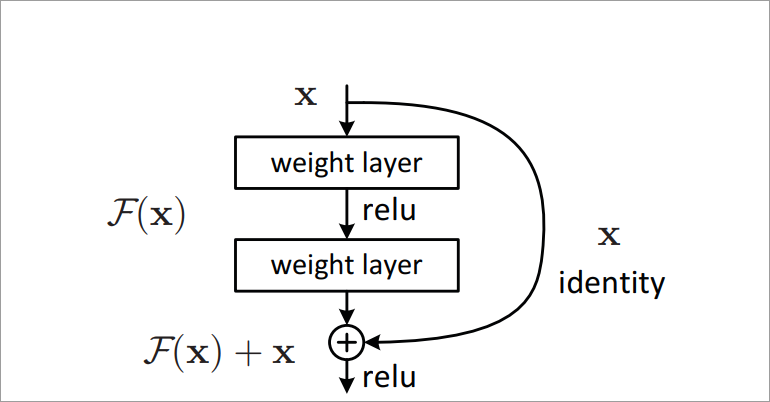
\includegraphics[width=0.6\textwidth]{informatica/bloque_resnet}
    \caption{Ejemplo de bloque residual. Imagen extraída de \cite{informatica:resnet_original_paper}}
    \label{img:ejemplo_bloque_resnet}
\end{figure}

En base a estos elementos, la arquitectura de nuestro modelo \textit{ResNet18} se describe gráficamente en la \imgref{img:arquitectura_resnet_18}. Notar que estamos modificando la última capa \textit{fully connected}, pasando de 1000 valores de salida a solo 9 (la dimensión de nuestro \textit{embedding}).

\begin{figure}[!hbt]
    \centering
    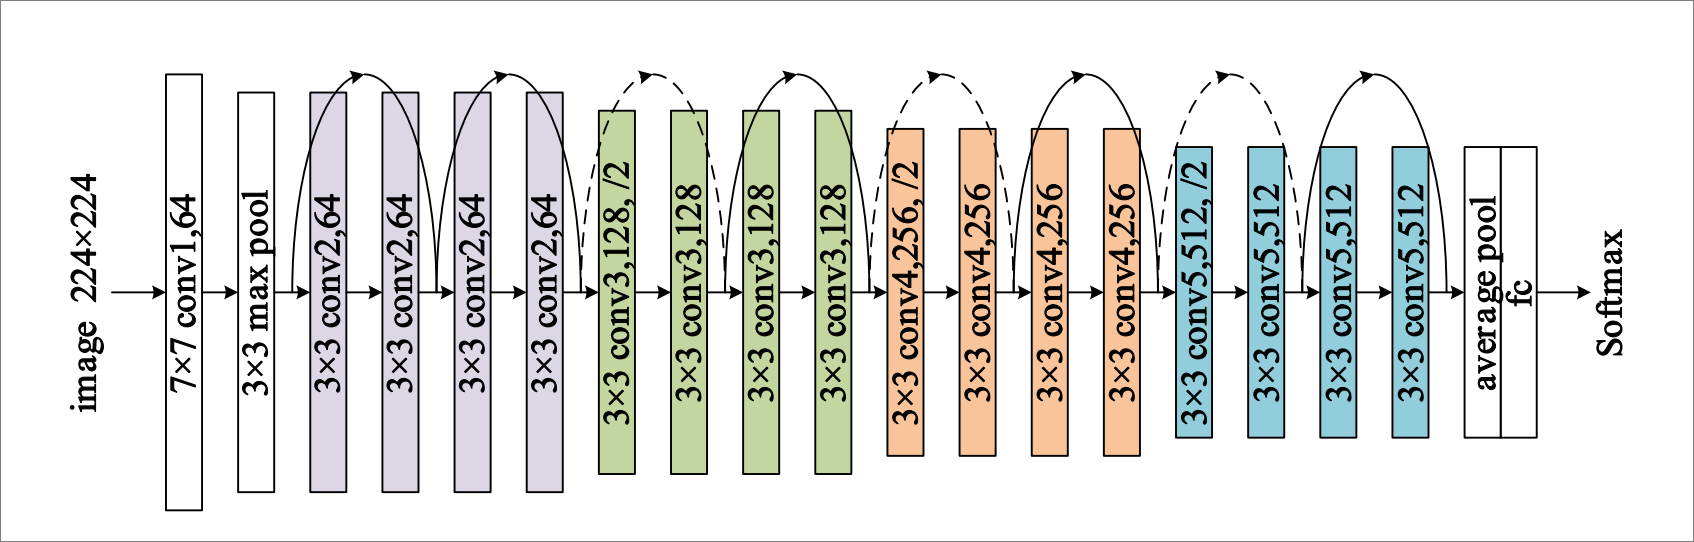
\includegraphics[width=1.0\textwidth]{informatica/resnet18_arch}
    \caption{Diagrama de la arquitectura \textit{ResNet18}. Las líneas continuas por encima de los bloques indican la conexión entre el inicio y final de un bloque residual. Las líneas discontinuas por encima de los bloques indican las \textit{skip connections}. Imagen extraída de \cite{informatica:resnet18_arch_web}}
    \label{img:arquitectura_resnet_18}
\end{figure}

\section{Entrenamiento del modelo} \label{isec:entrenamiento_mejor_modelo}

Entrenamos el modelo usando los hiperparámetros indicados en \tableref{table:hp_escogidos}. Además, especificamos los siguientes hiperparámetros:

\begin{itemize}
    \item Función de pérdida: \textit{batch hard} con sumandos activos, es decir, $\mathcal{L}_{BH \neq 0}$. Elegimos esta función en base a la experimentación realizada sobre los \textit{datasets} previos a \textit{CACD} y \textit{FG-Net}.
    \item Épocas de entrenamiento: una única época de entrenamiento. El conjunto de entrenamiento \textit{CACD} es lo suficientemente grande como para entrenar en una sola época. Tomamos esta decisión en base a experimentos previos y a los propios resultados de este entrenamiento..
    \item Técnica de Aumentado de Datos: \textit{lazy}. Esta variante permite que no saturemos la memoria disponible. De otra forma, en algunos experimentos obtenemos errores al ocurrir dicha saturación de la memoria. De otra forma, en algunos experimentos obtenemos errores al ocurrir dicha saturación de la memoria.
    \item Usamos el 80\% del \textit{dataset} \textit{CACD} para entrenar, y el 20\% restante como conjunto de validación.
\end{itemize}

El proceso de entrenamiento puede estudiarse a partir de las métricas que se muestran en \imgref{img:metricas_entrenamiento}. Al finalizar el entrenamiento, evaluamos distintas métricas sobre el conjunto \textit{FG-Net}. Estos resultados se muestran en la \tableref{table:resultados_sobre_fg_net}.

\begin{figure}[!hbtp]
    \centering
    \begin{subfigure}[t]{0.45\textwidth}
        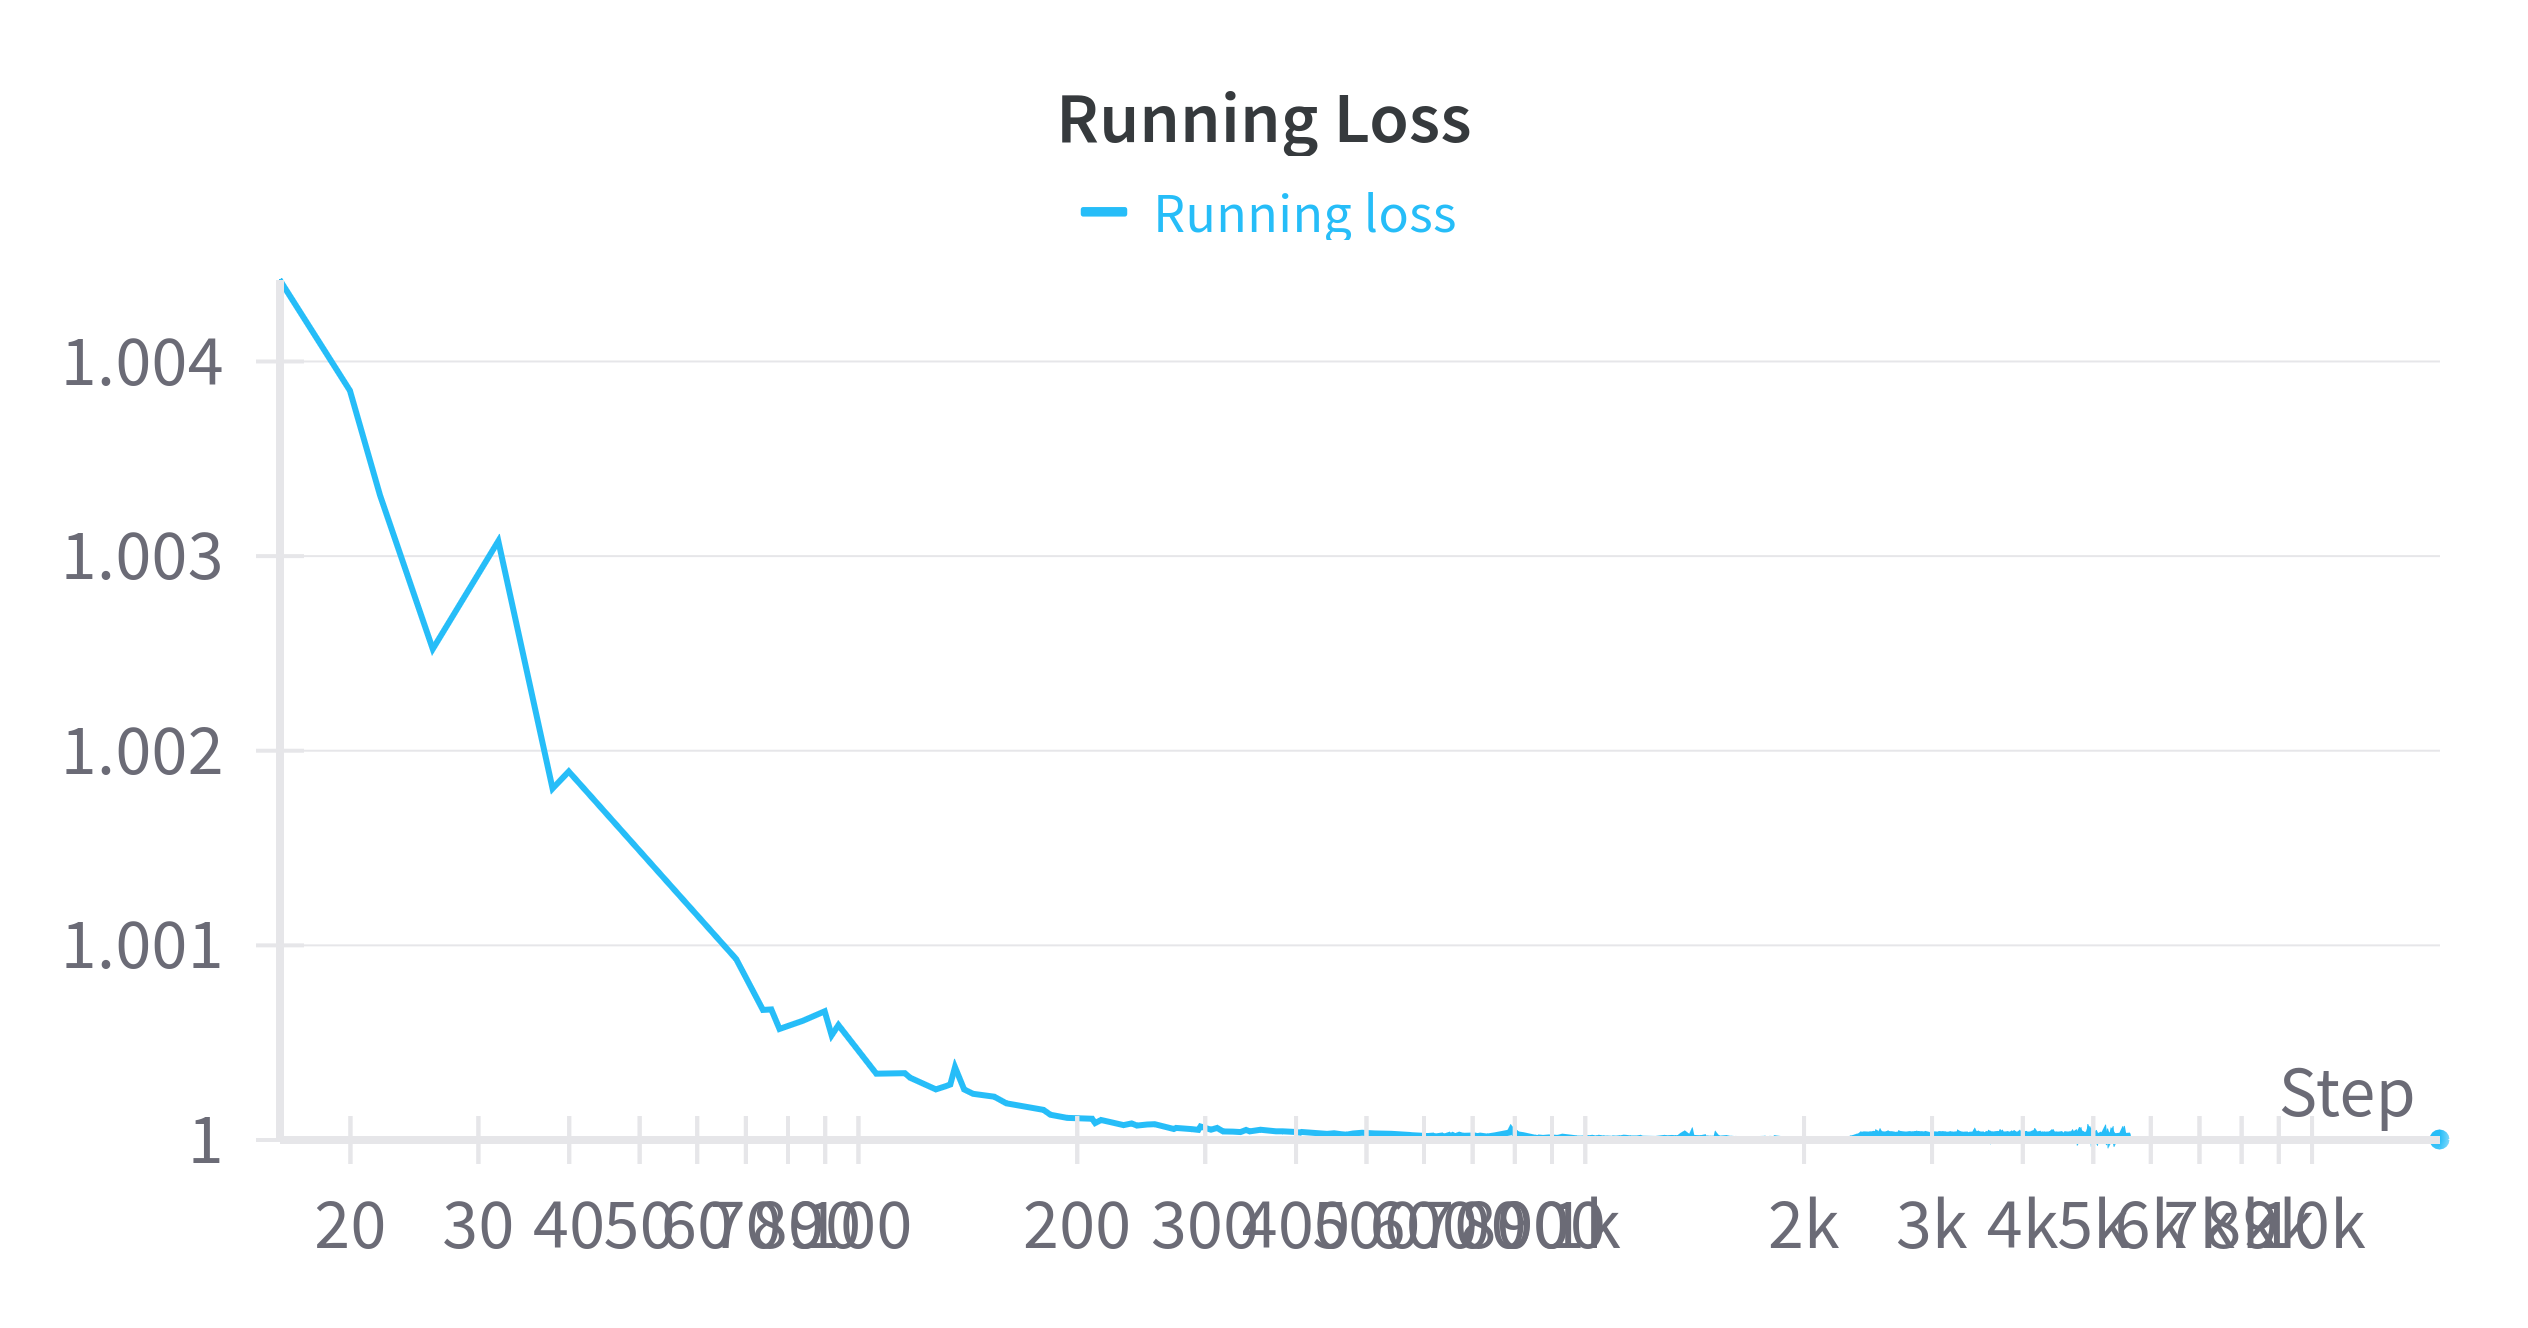
\includegraphics[width=1.0\textwidth]{informatica/wandb/entrenamiento_principal/running_loss}
        \caption{Error de entrenamiento tipo \entrecomillado{running}}
    \end{subfigure}
    \begin{subfigure}[t]{0.45\textwidth}
        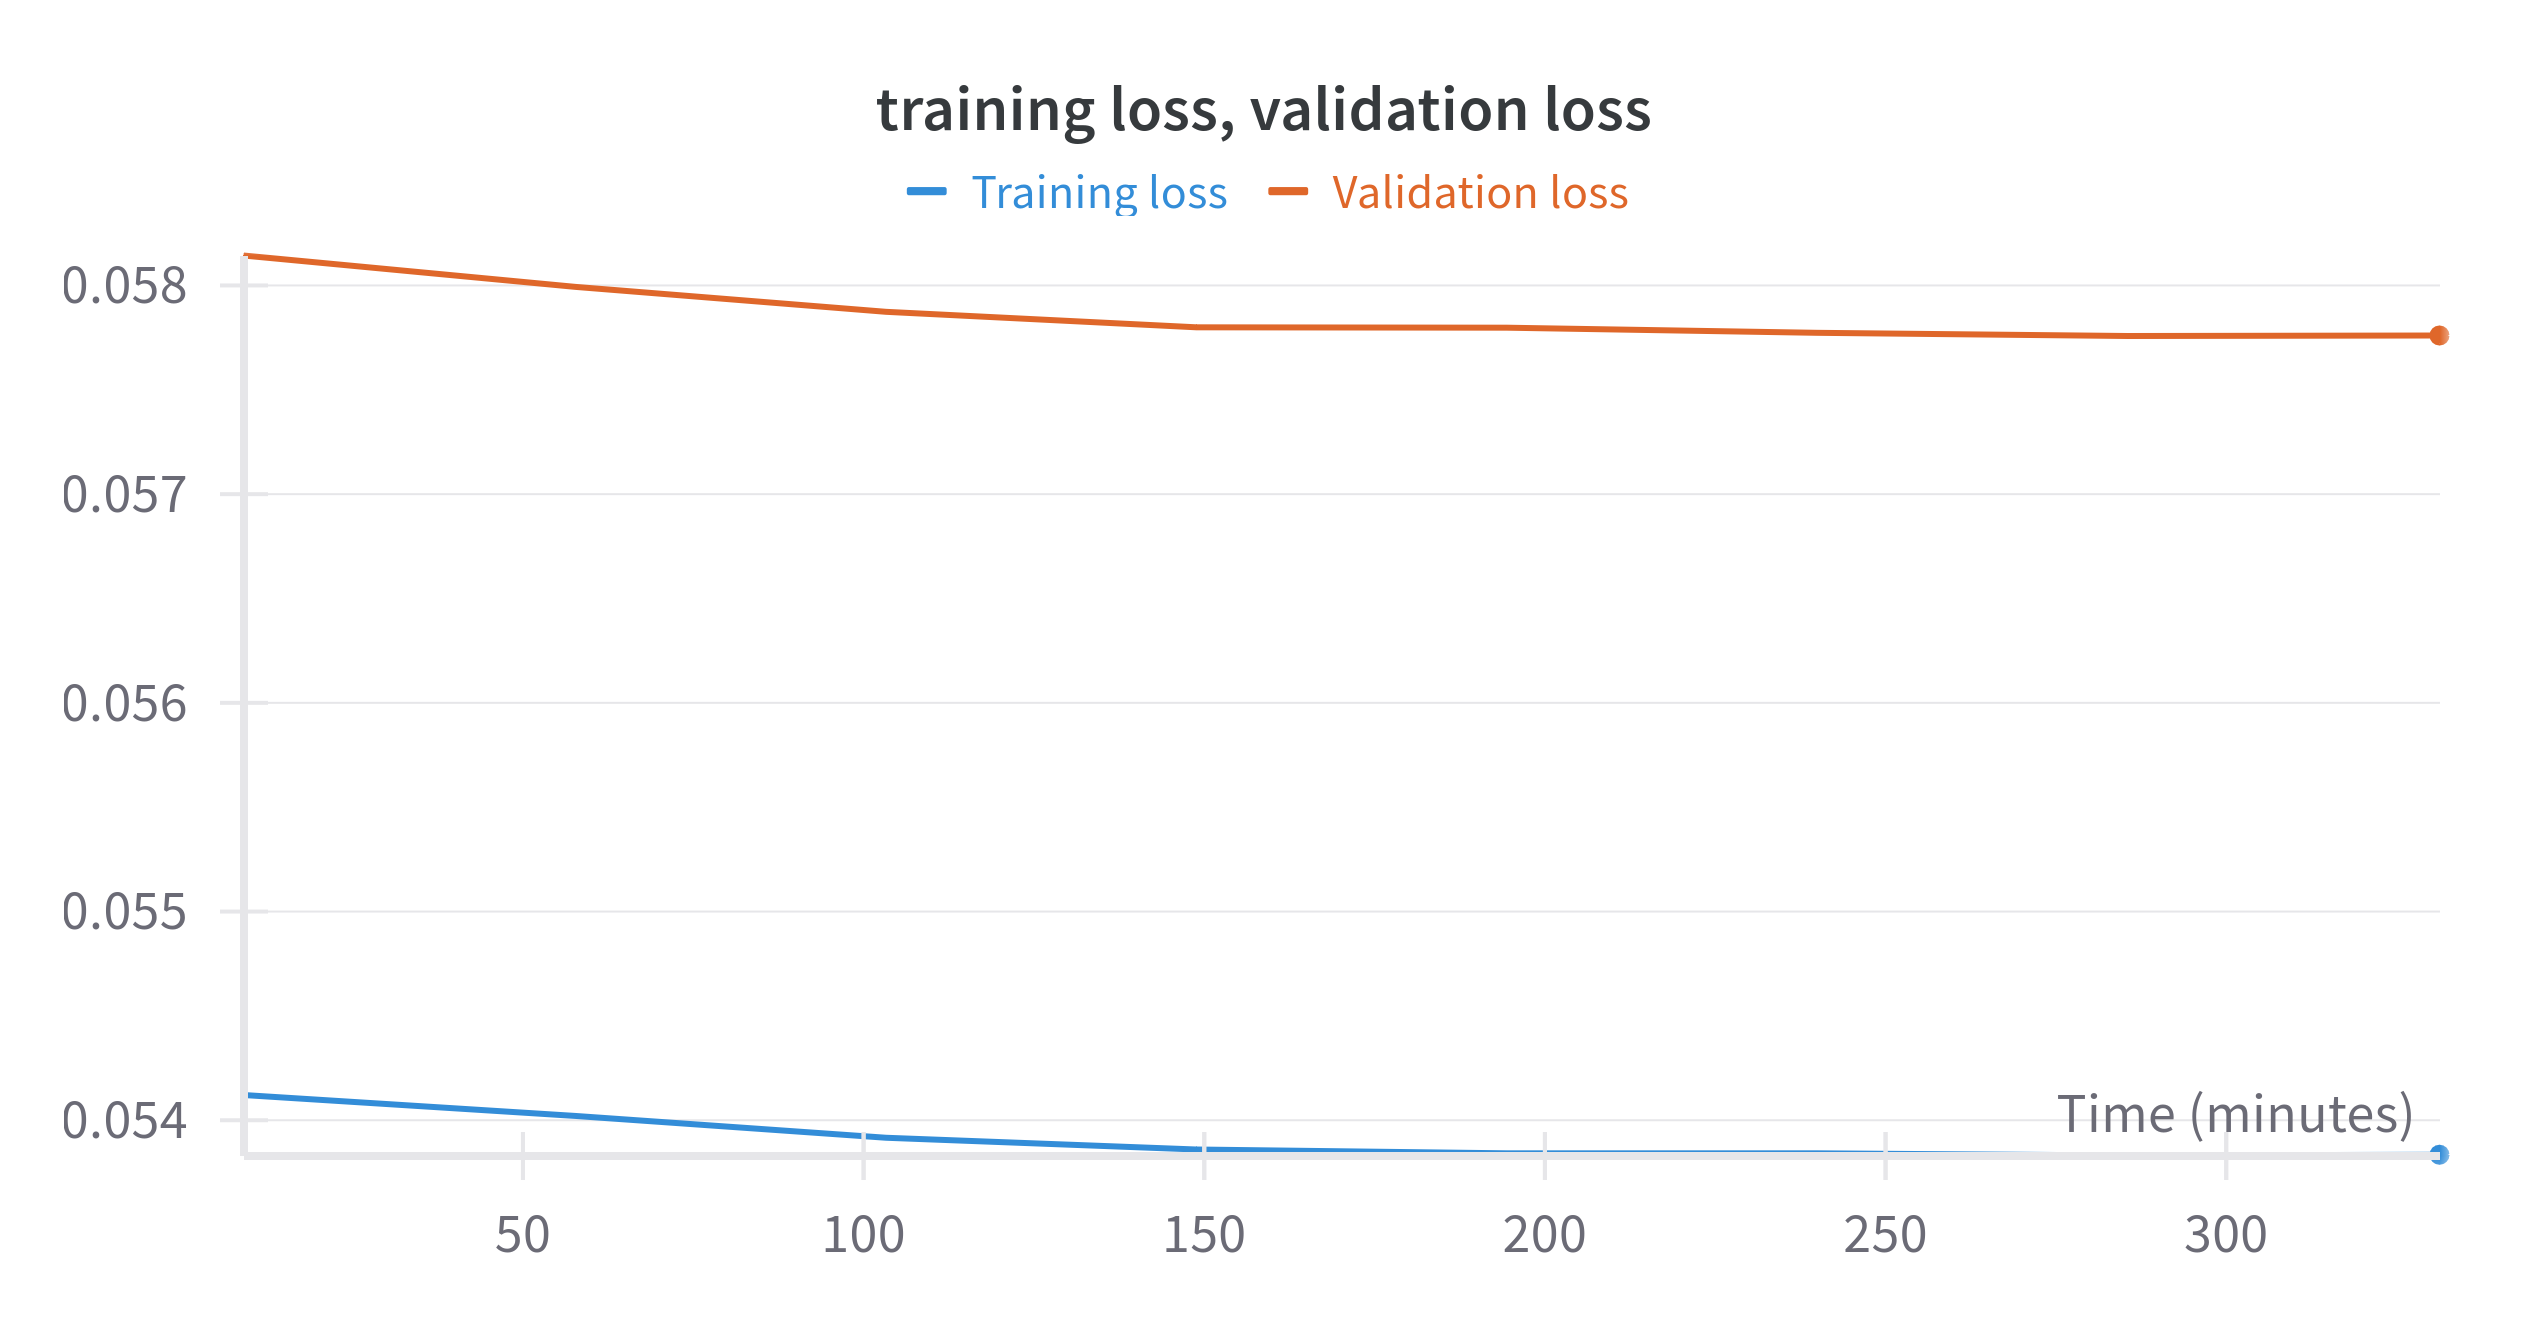
\includegraphics[width=1.0\textwidth]{informatica/wandb/entrenamiento_principal/manual_loss}
        \caption{Error de entrenamiento}
    \end{subfigure}

    \begin{subfigure}[t]{0.45\textwidth}
        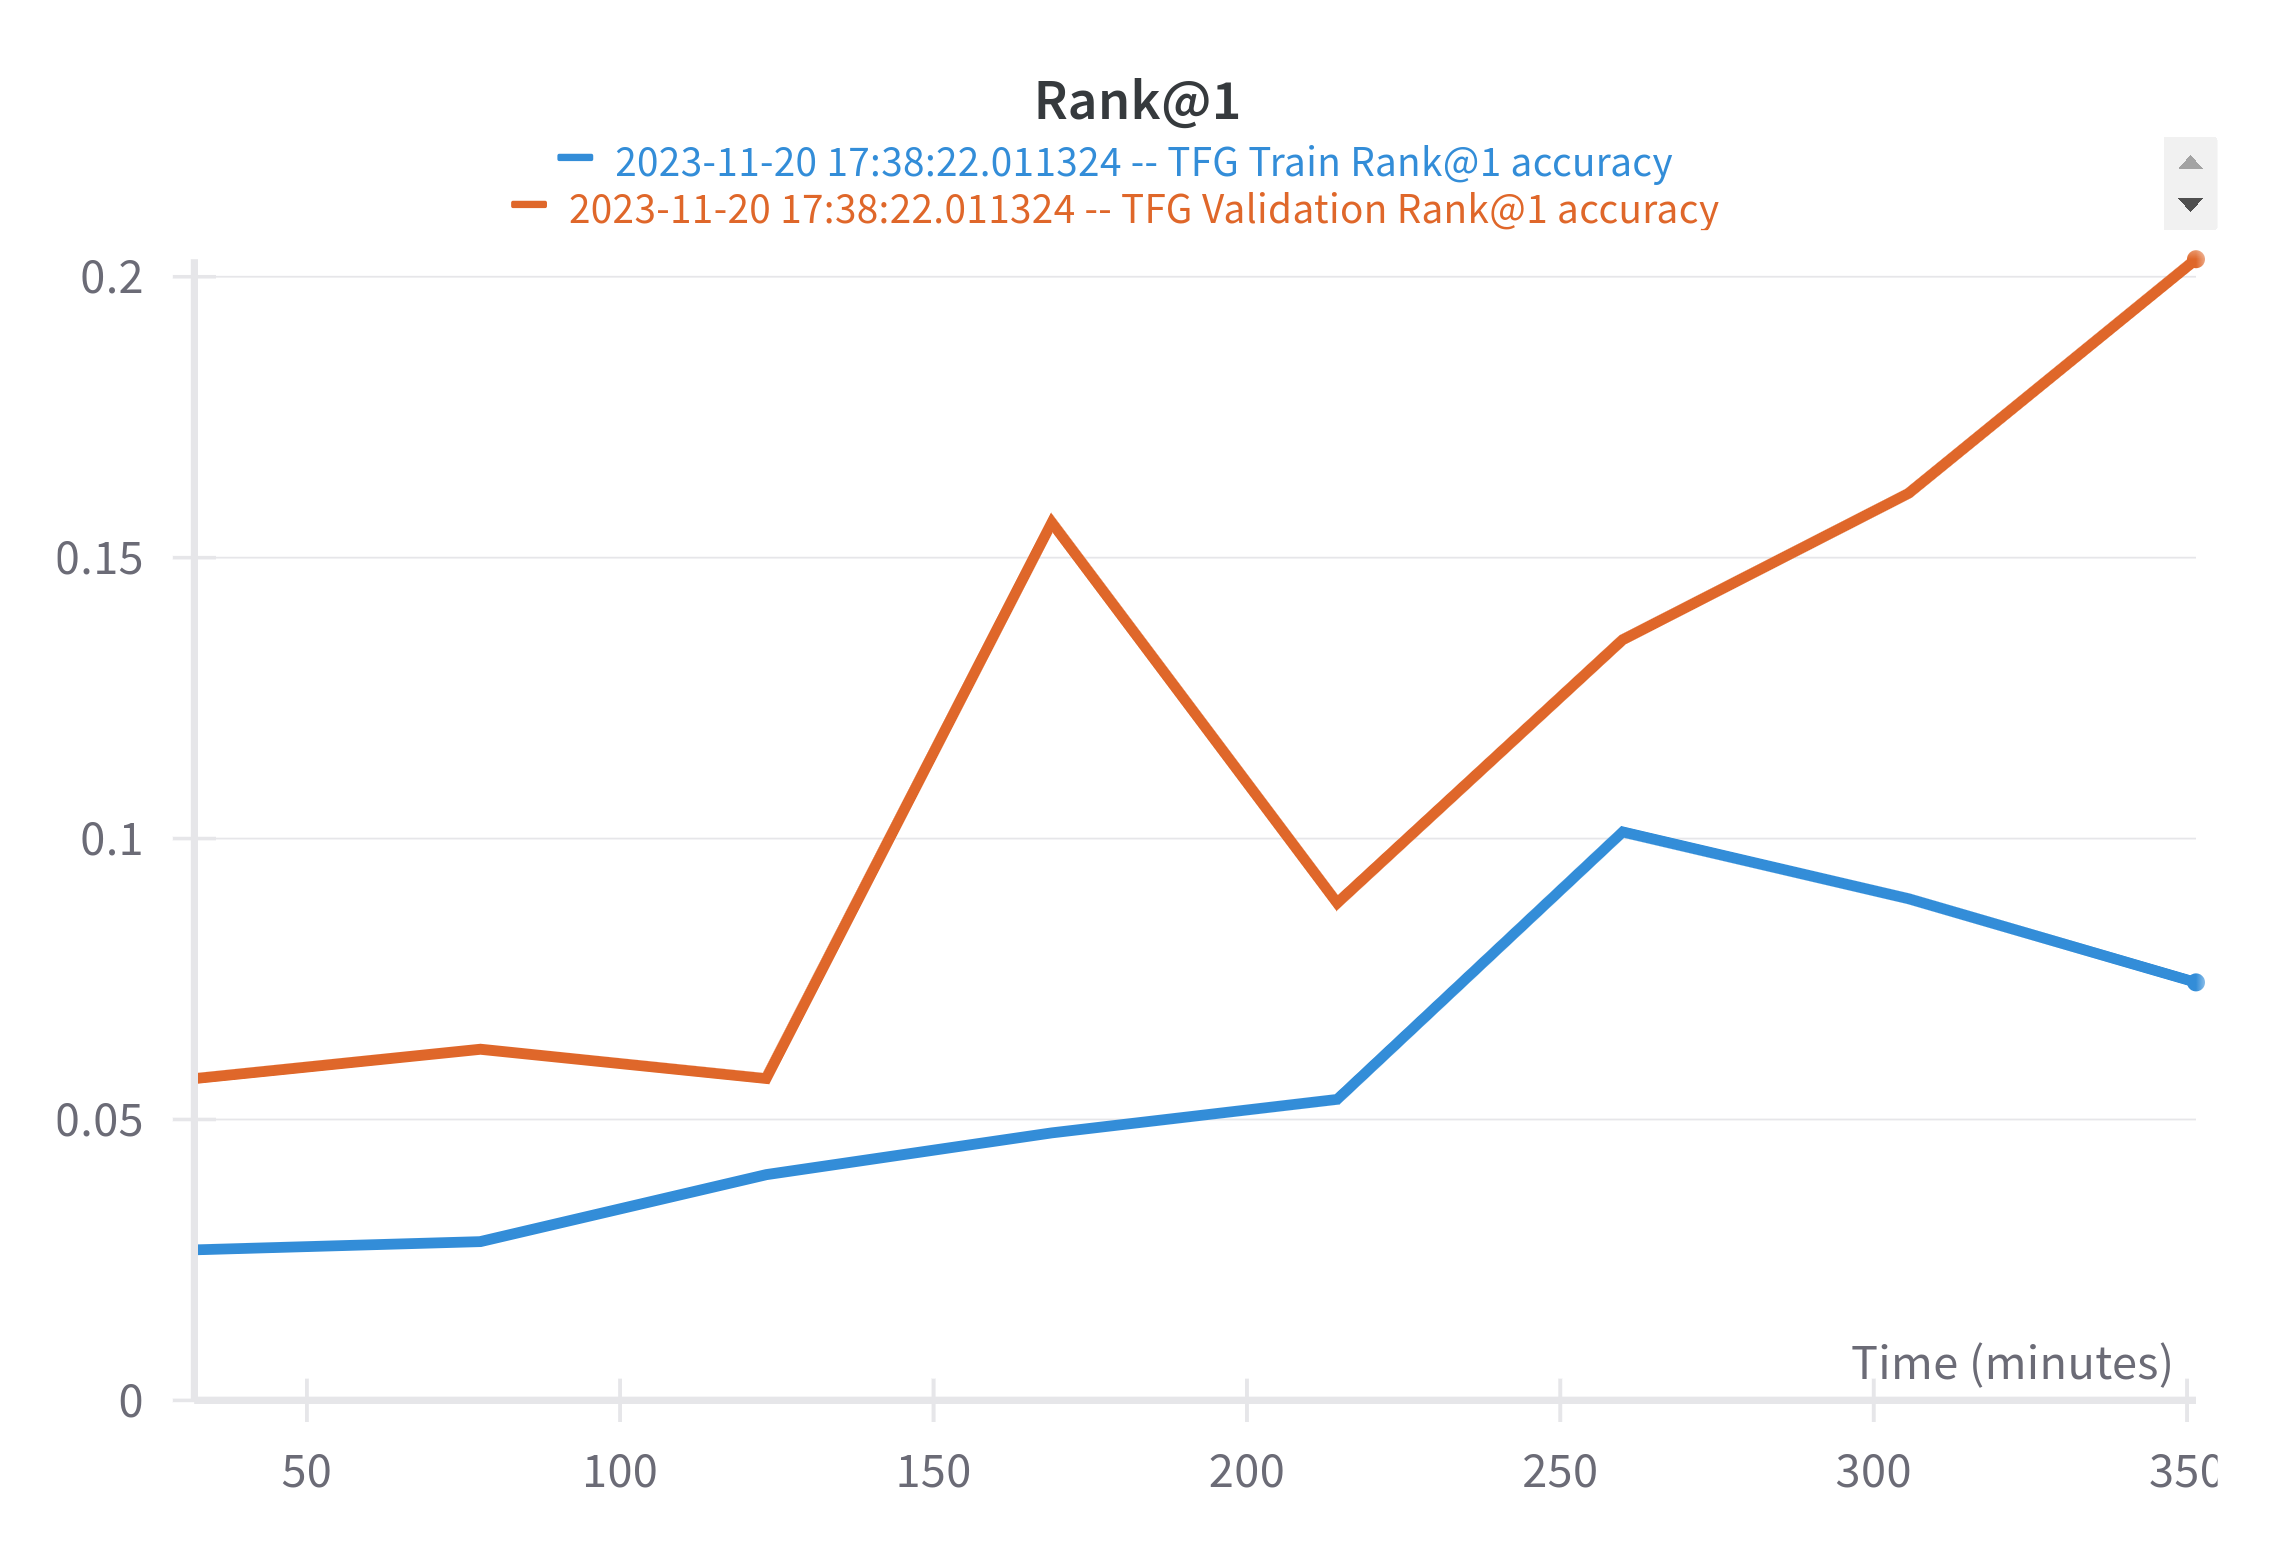
\includegraphics[width=1.0\textwidth]{informatica/wandb/entrenamiento_principal/rank@1}
        \caption{\textit{Rank@1 Accuracy}}
    \end{subfigure}
    \begin{subfigure}[t]{0.45\textwidth}
        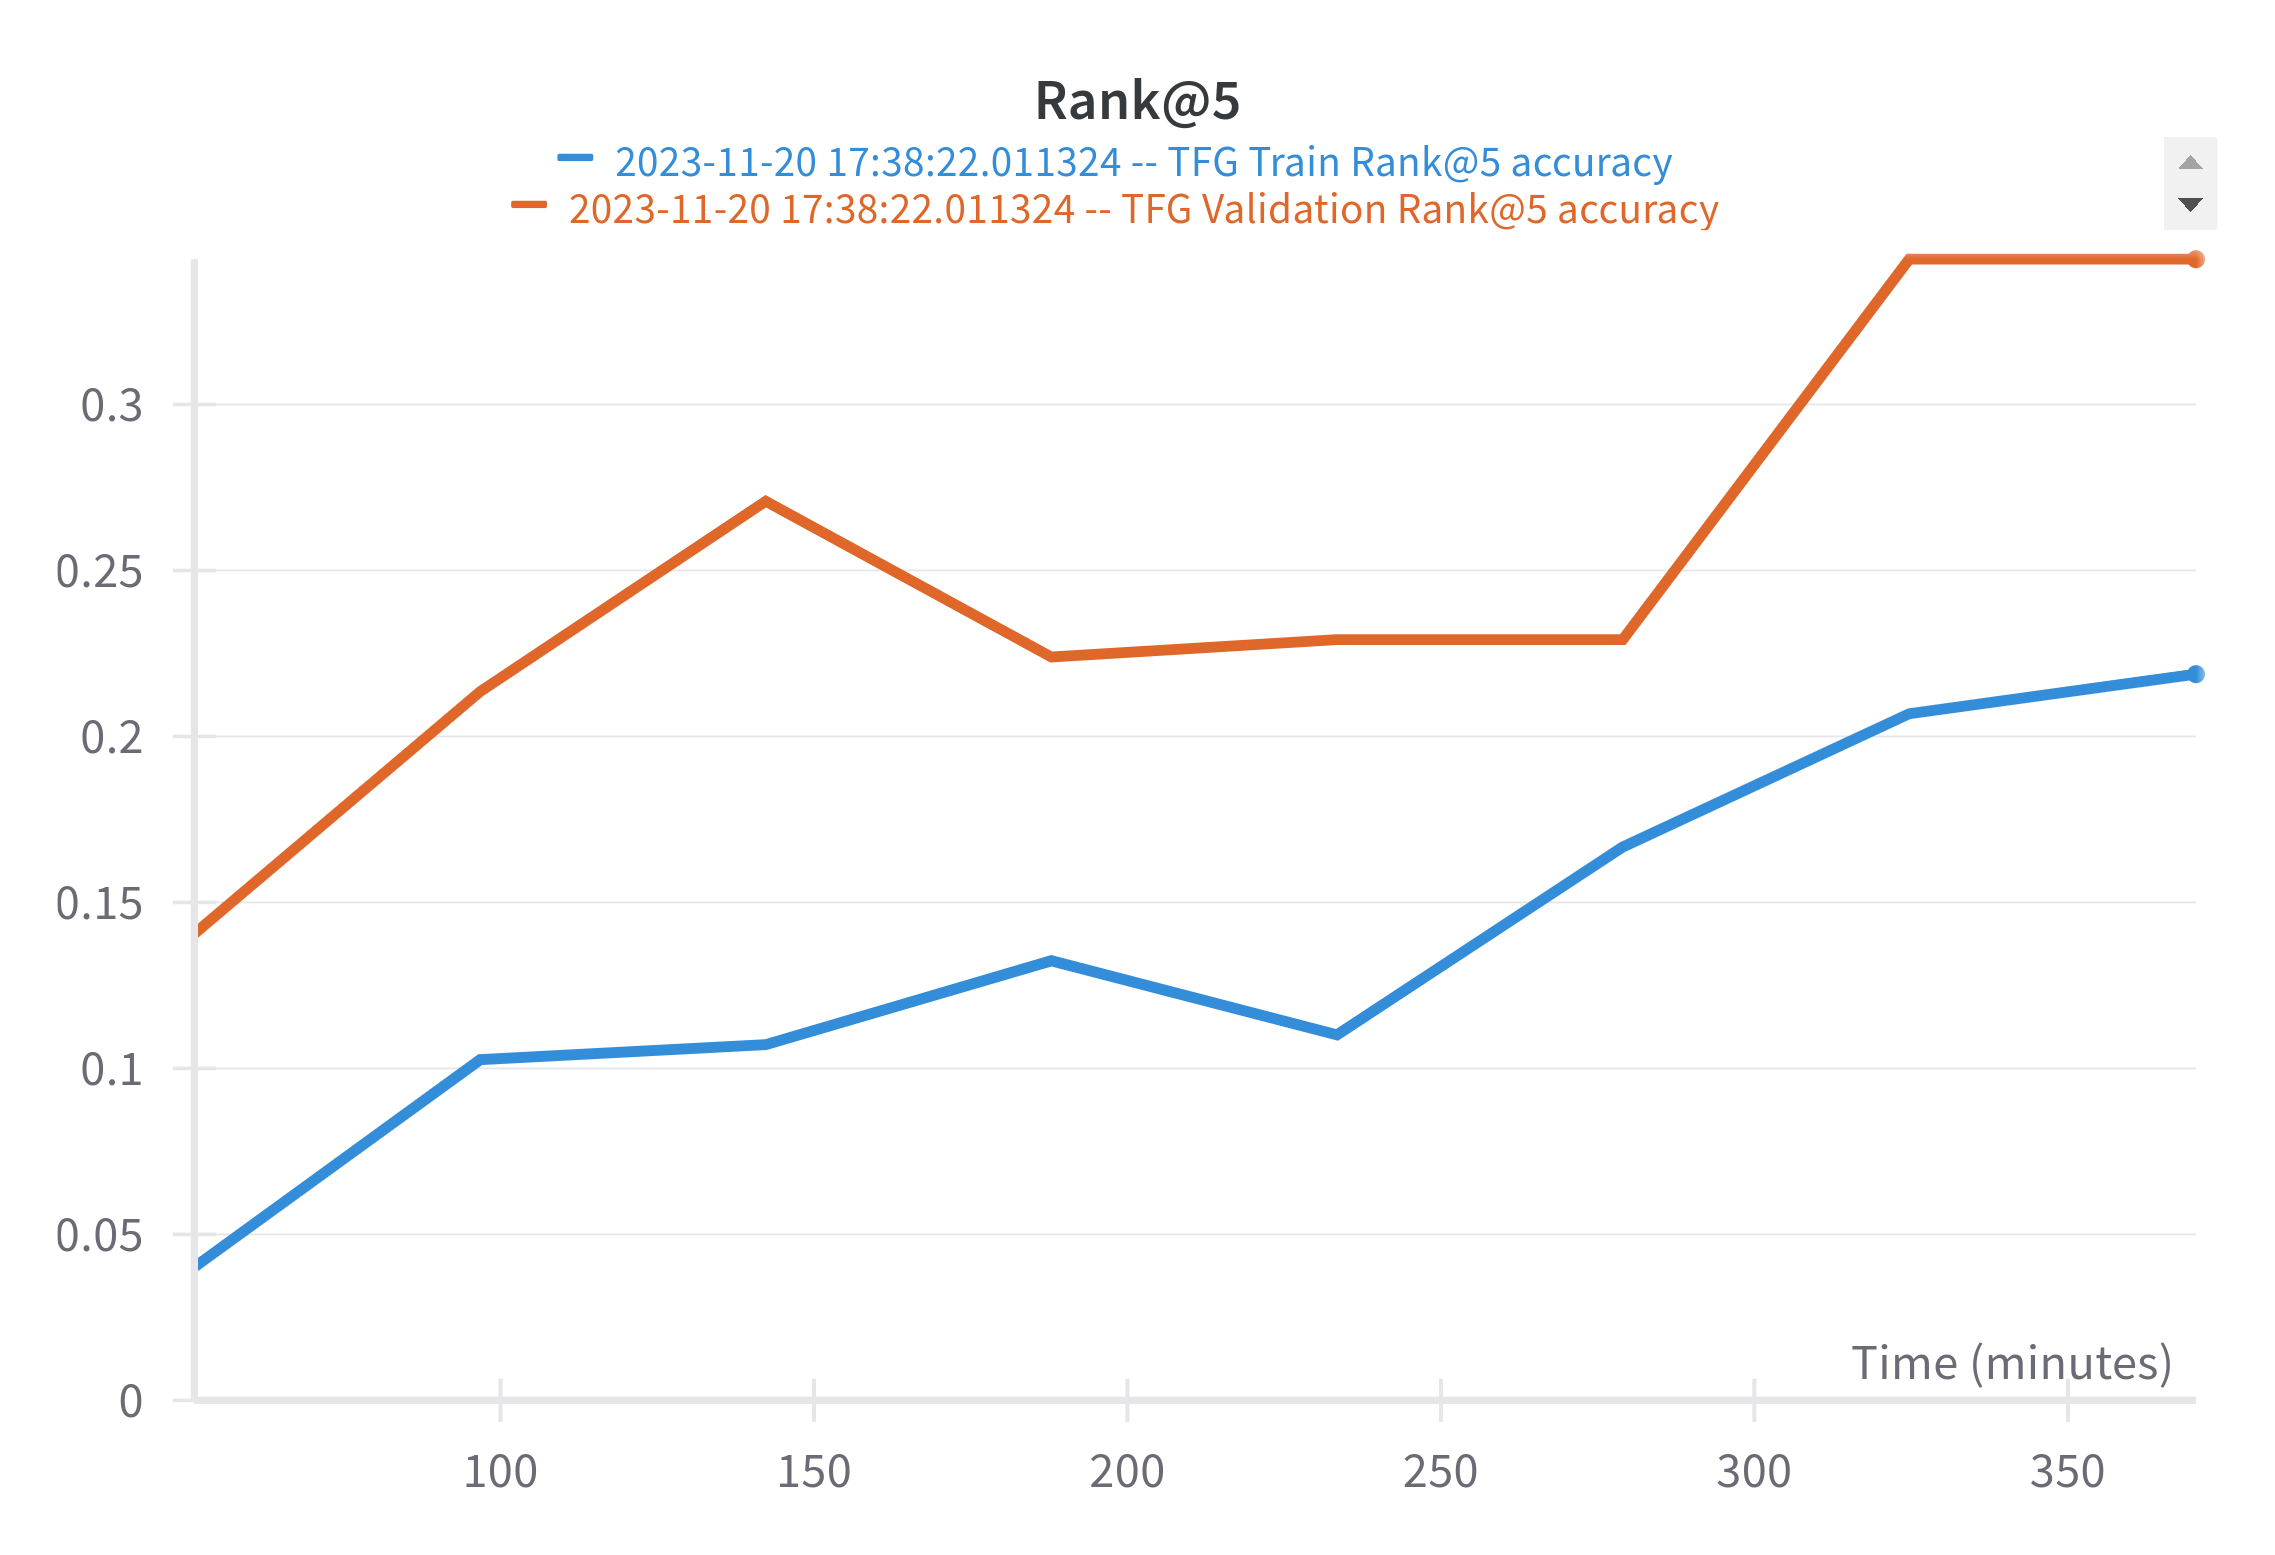
\includegraphics[width=1.0\textwidth]{informatica/wandb/entrenamiento_principal/rank@5}
        \caption{\textit{Rank@5 Accuracy}}
    \end{subfigure}

    \begin{subfigure}[t]{0.45\textwidth}
        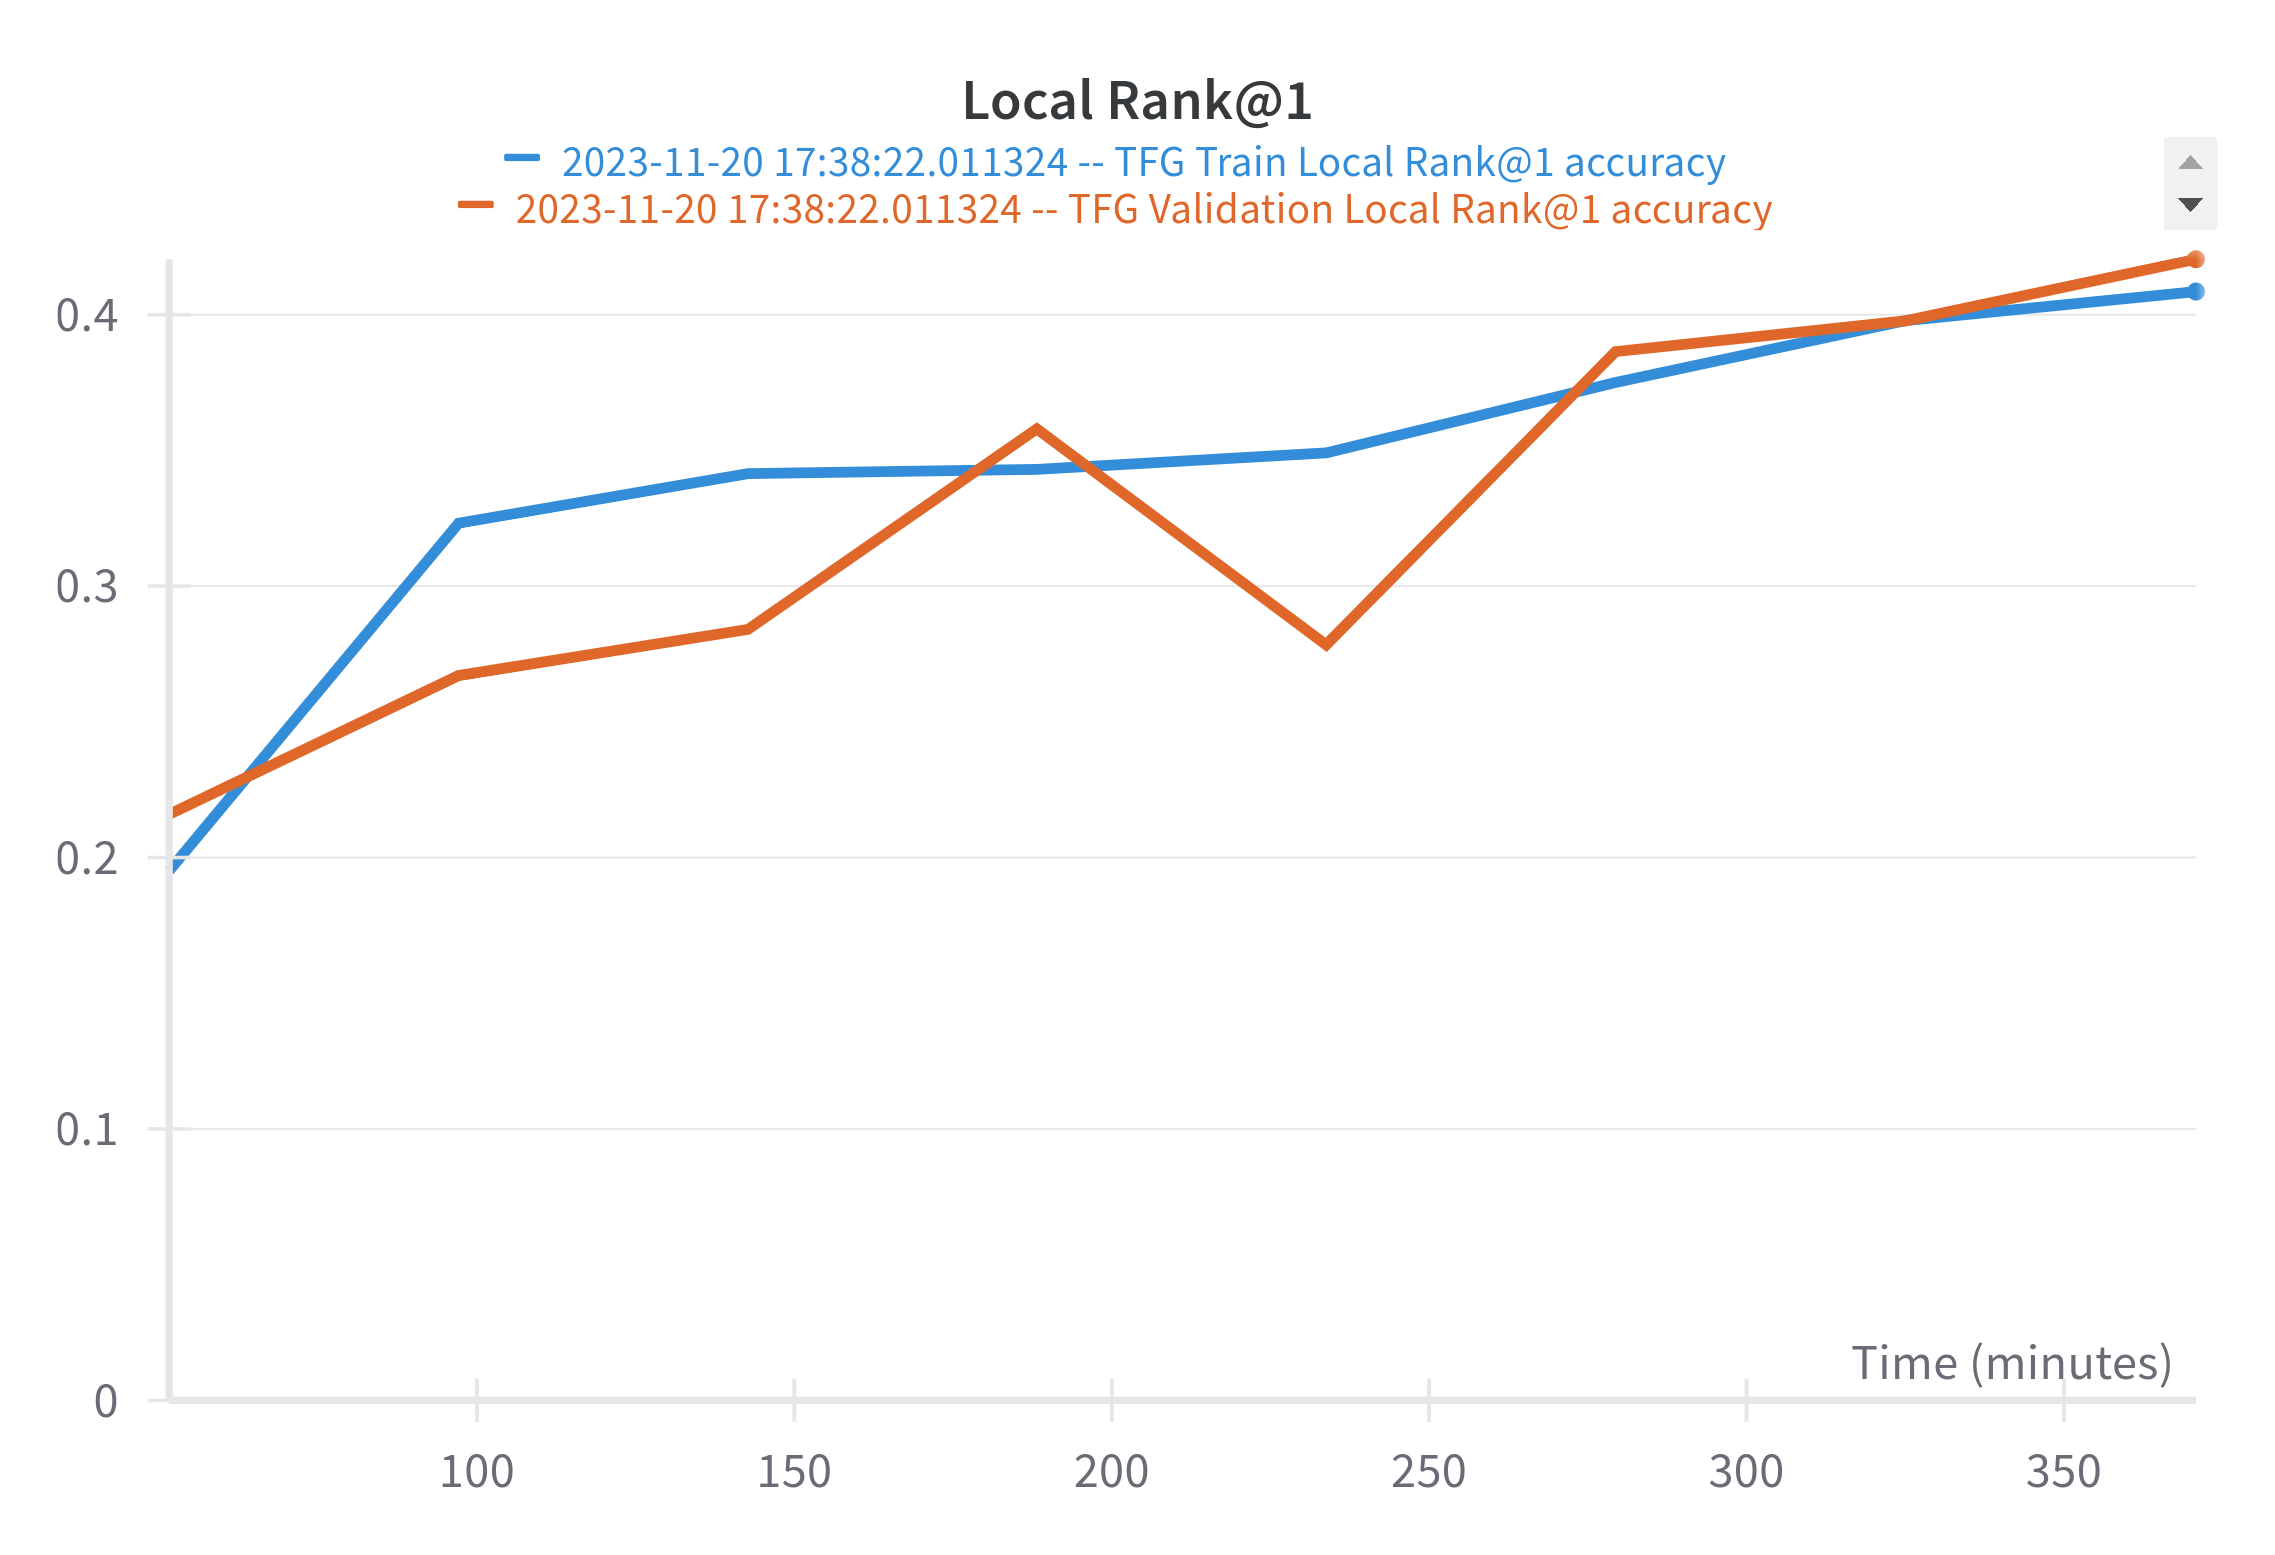
\includegraphics[width=1.0\textwidth]{informatica/wandb/entrenamiento_principal/local_rank@1}
        \caption{\textit{Rank@1 Accuracy}}
    \end{subfigure}
    \begin{subfigure}[t]{0.45\textwidth}
        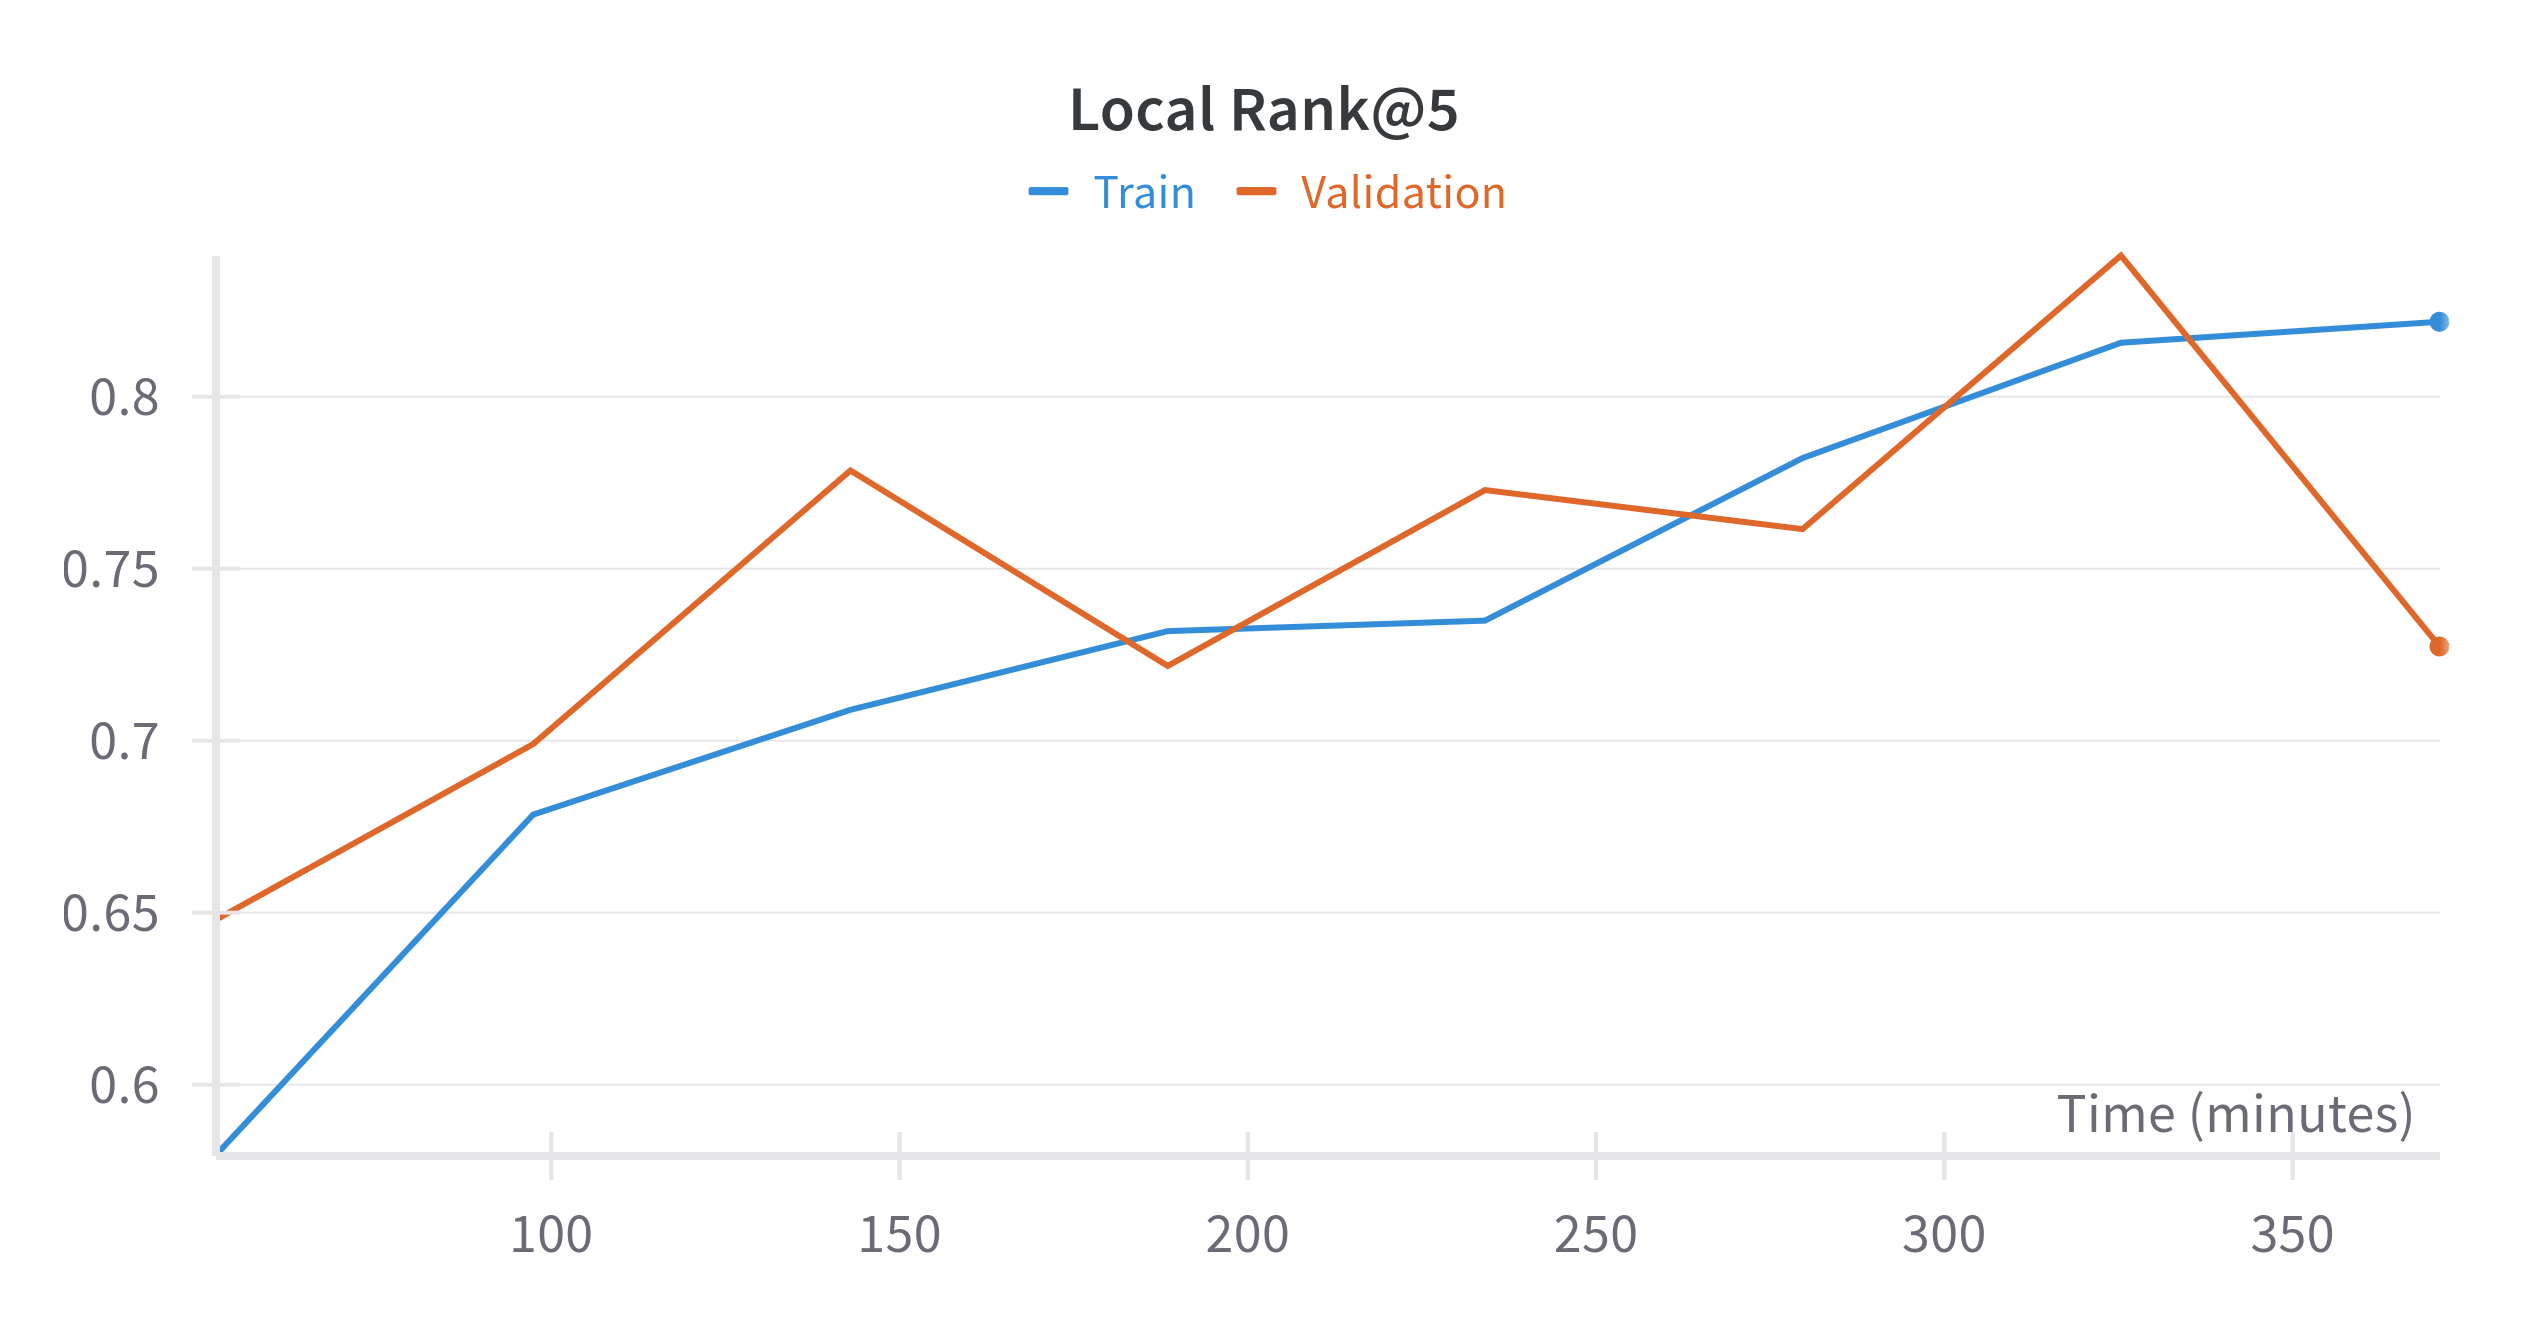
\includegraphics[width=1.0\textwidth]{informatica/wandb/entrenamiento_principal/local_rank@5}
        \caption{\textit{Local Rank@5 Accuracy}}
    \end{subfigure}

    \begin{subfigure}[t]{0.45\textwidth}
        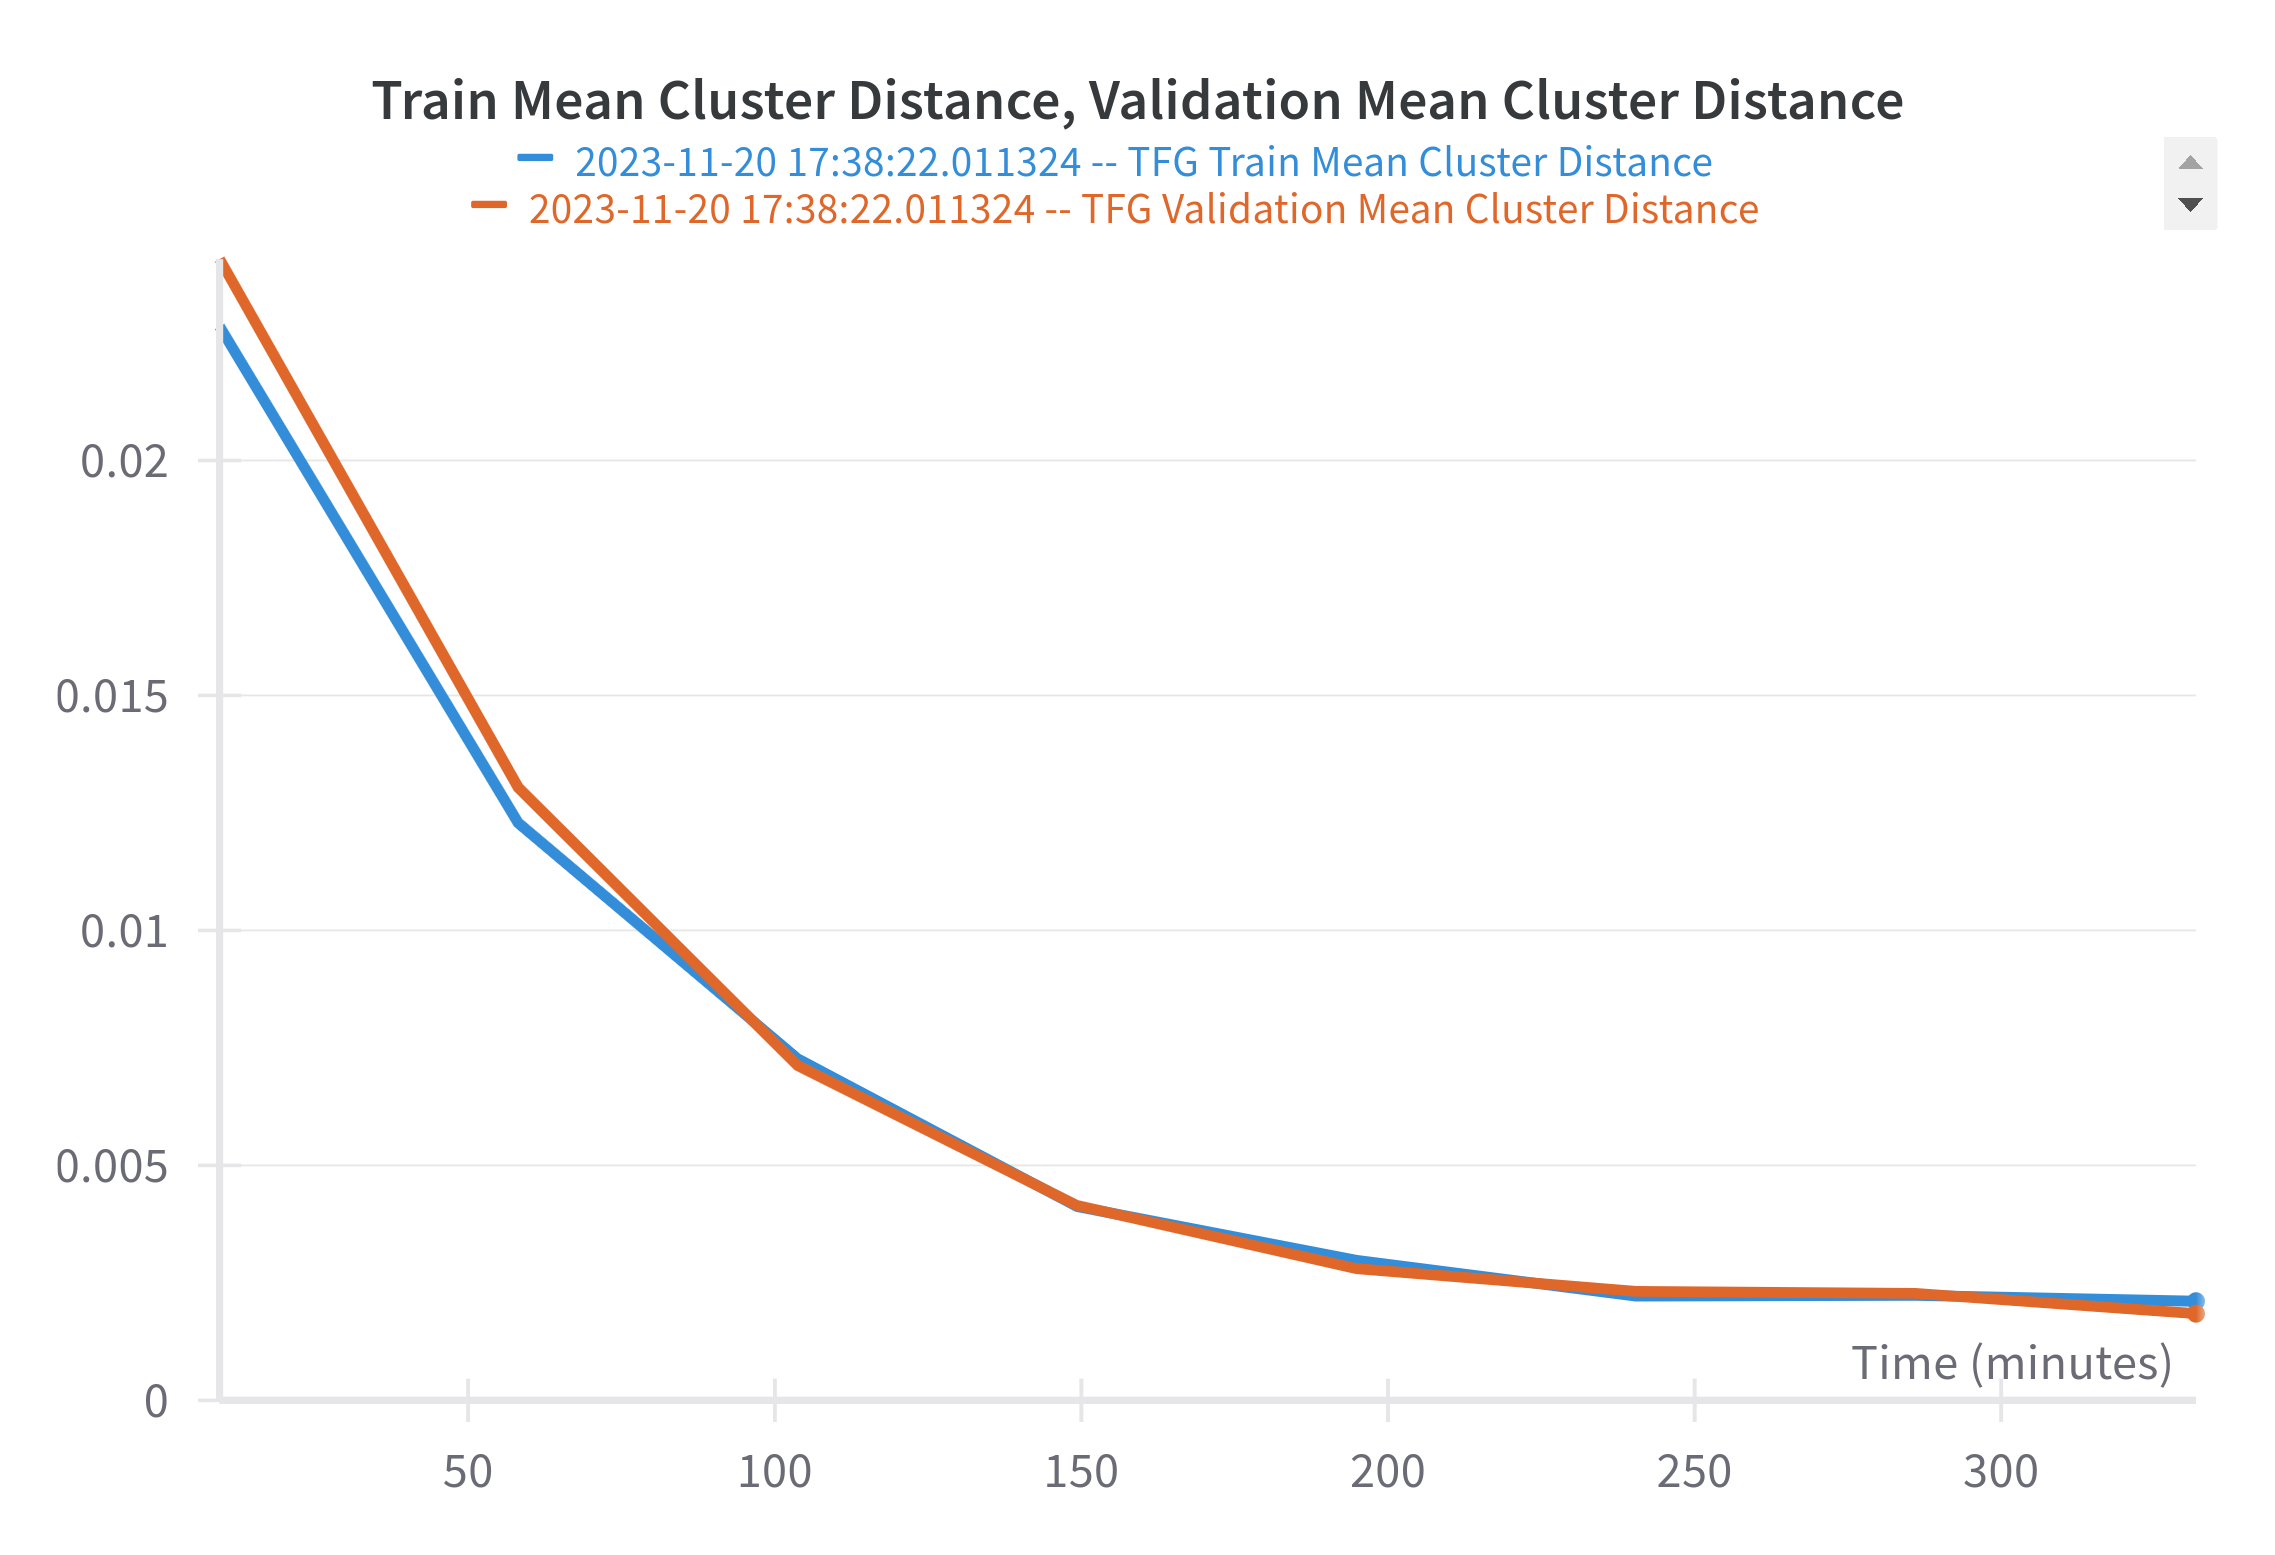
\includegraphics[width=1.0\textwidth]{informatica/wandb/entrenamiento_principal/intracluster_distance}
        \caption{Distanca \textit{intracluster} media}
    \end{subfigure}
    \begin{subfigure}[t]{0.45\textwidth}
        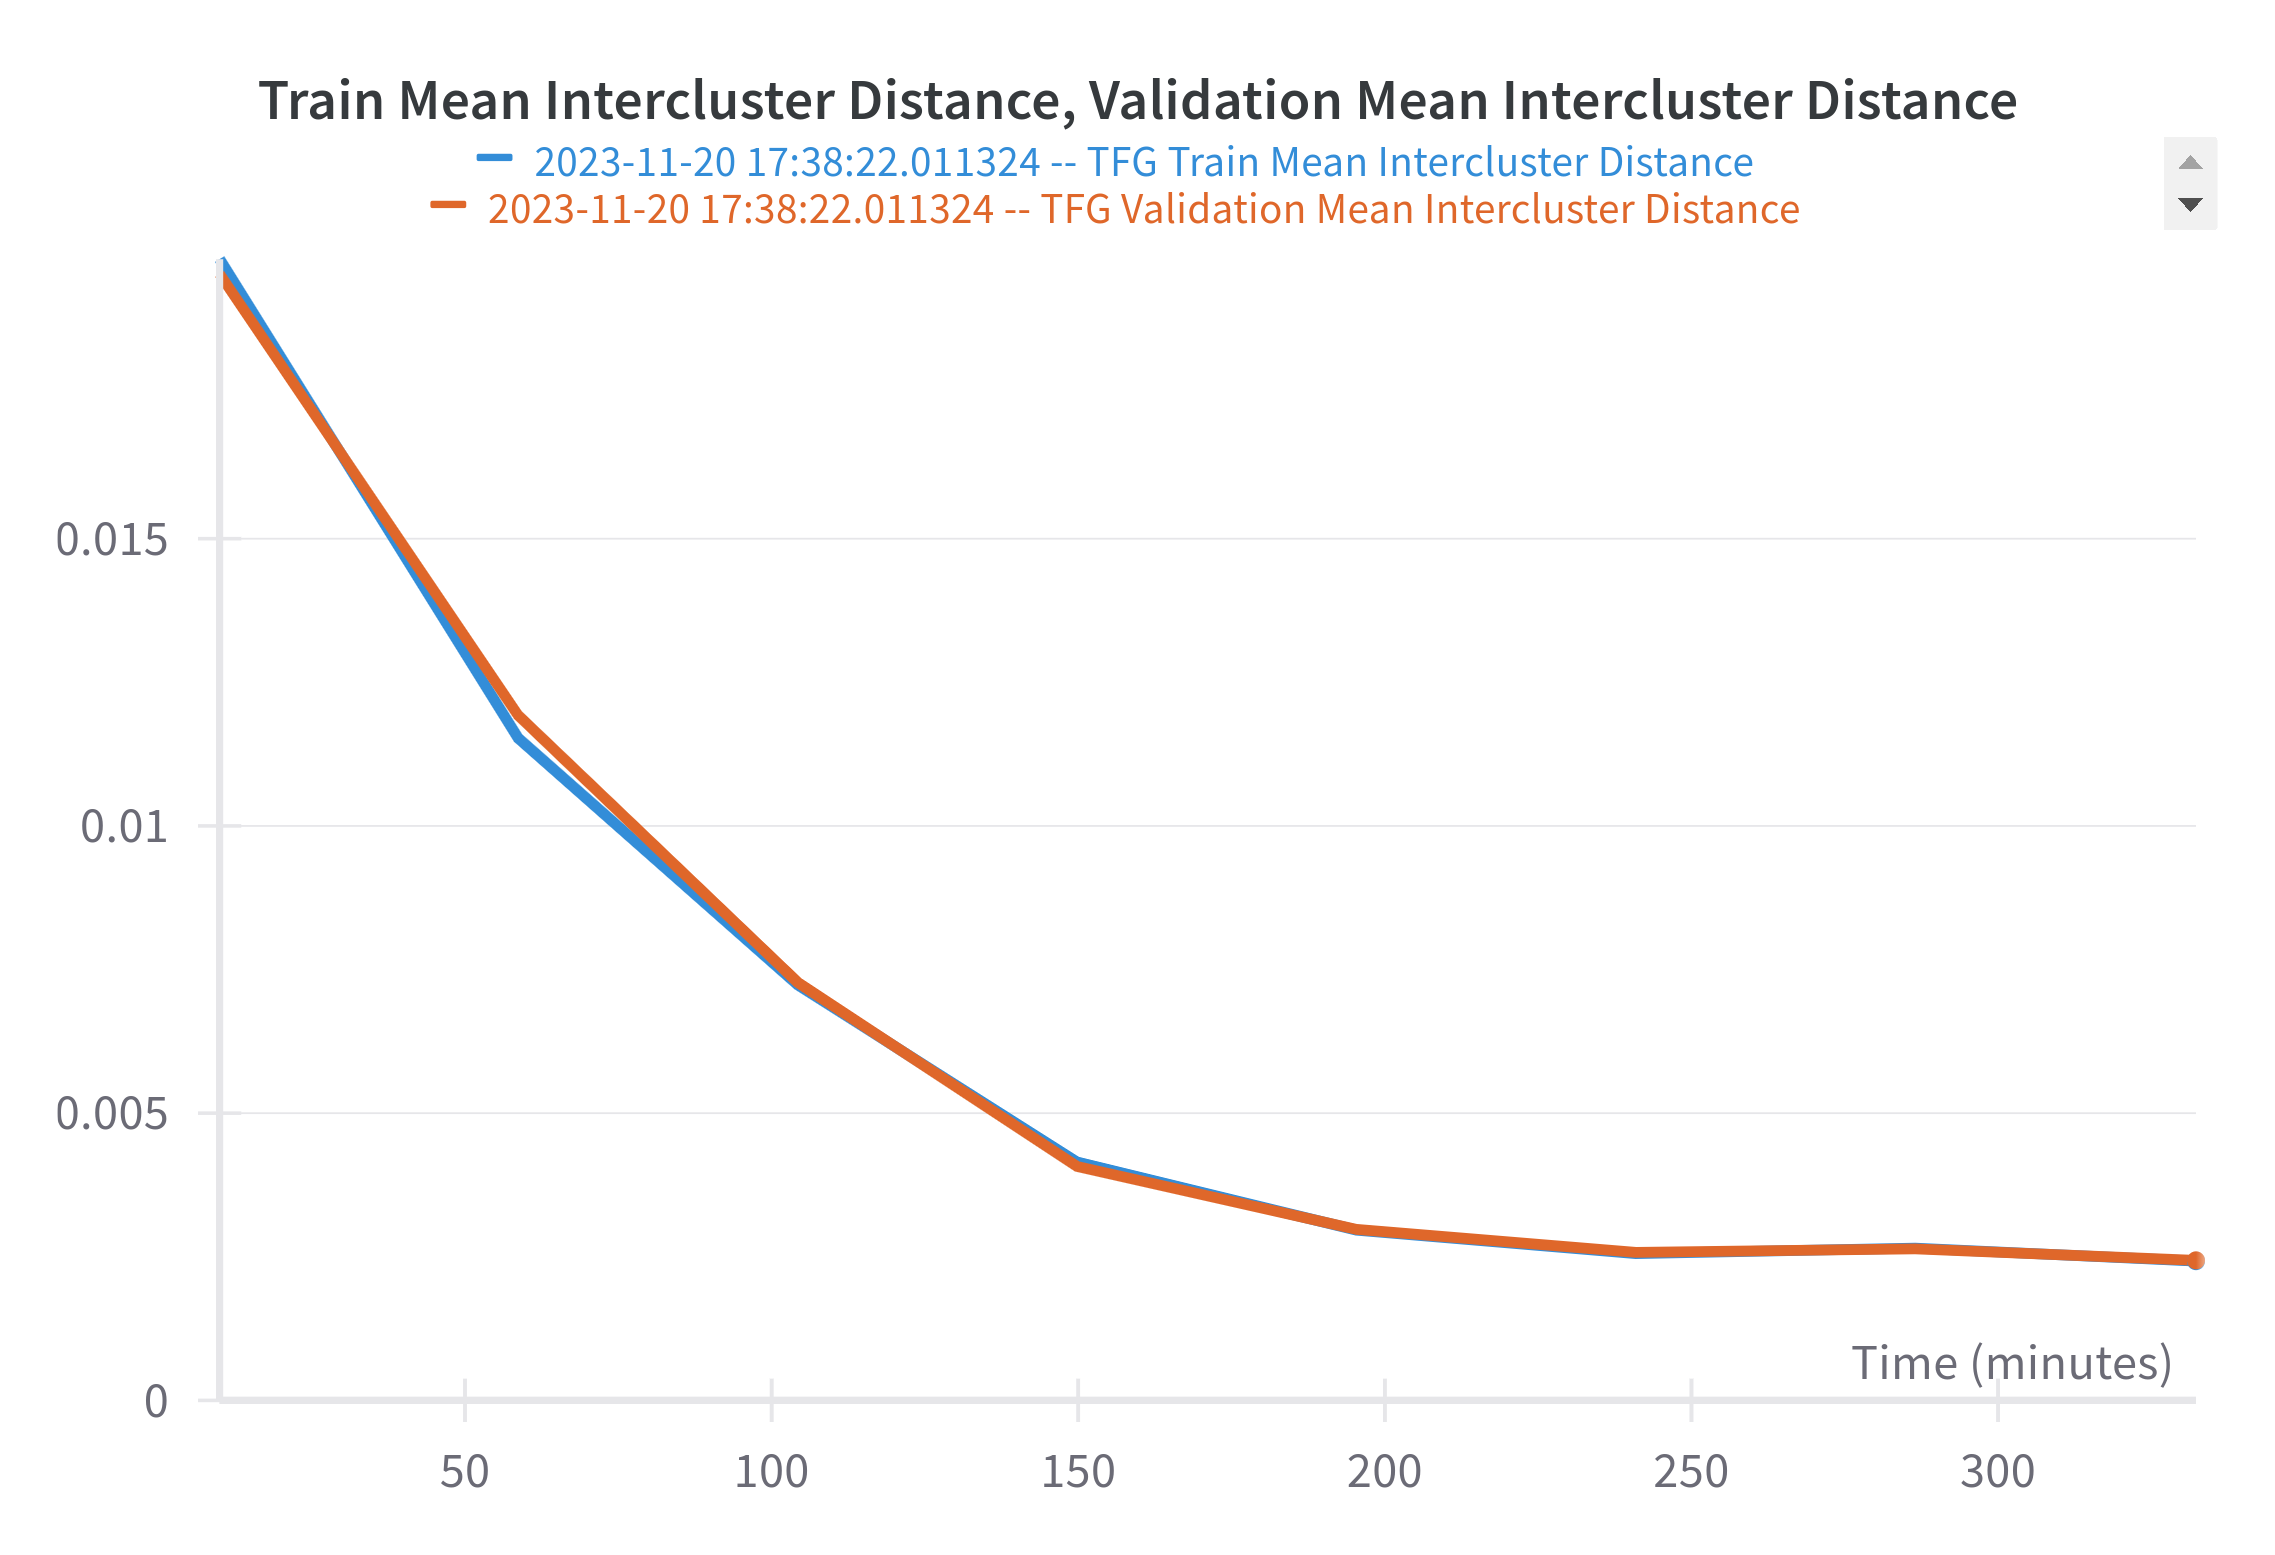
\includegraphics[width=1.0\textwidth]{informatica/wandb/entrenamiento_principal/intercluster_distance}
        \caption{Distancia \textit{intercluster} media}
    \end{subfigure}

    \begin{subfigure}[t]{0.45\textwidth}
        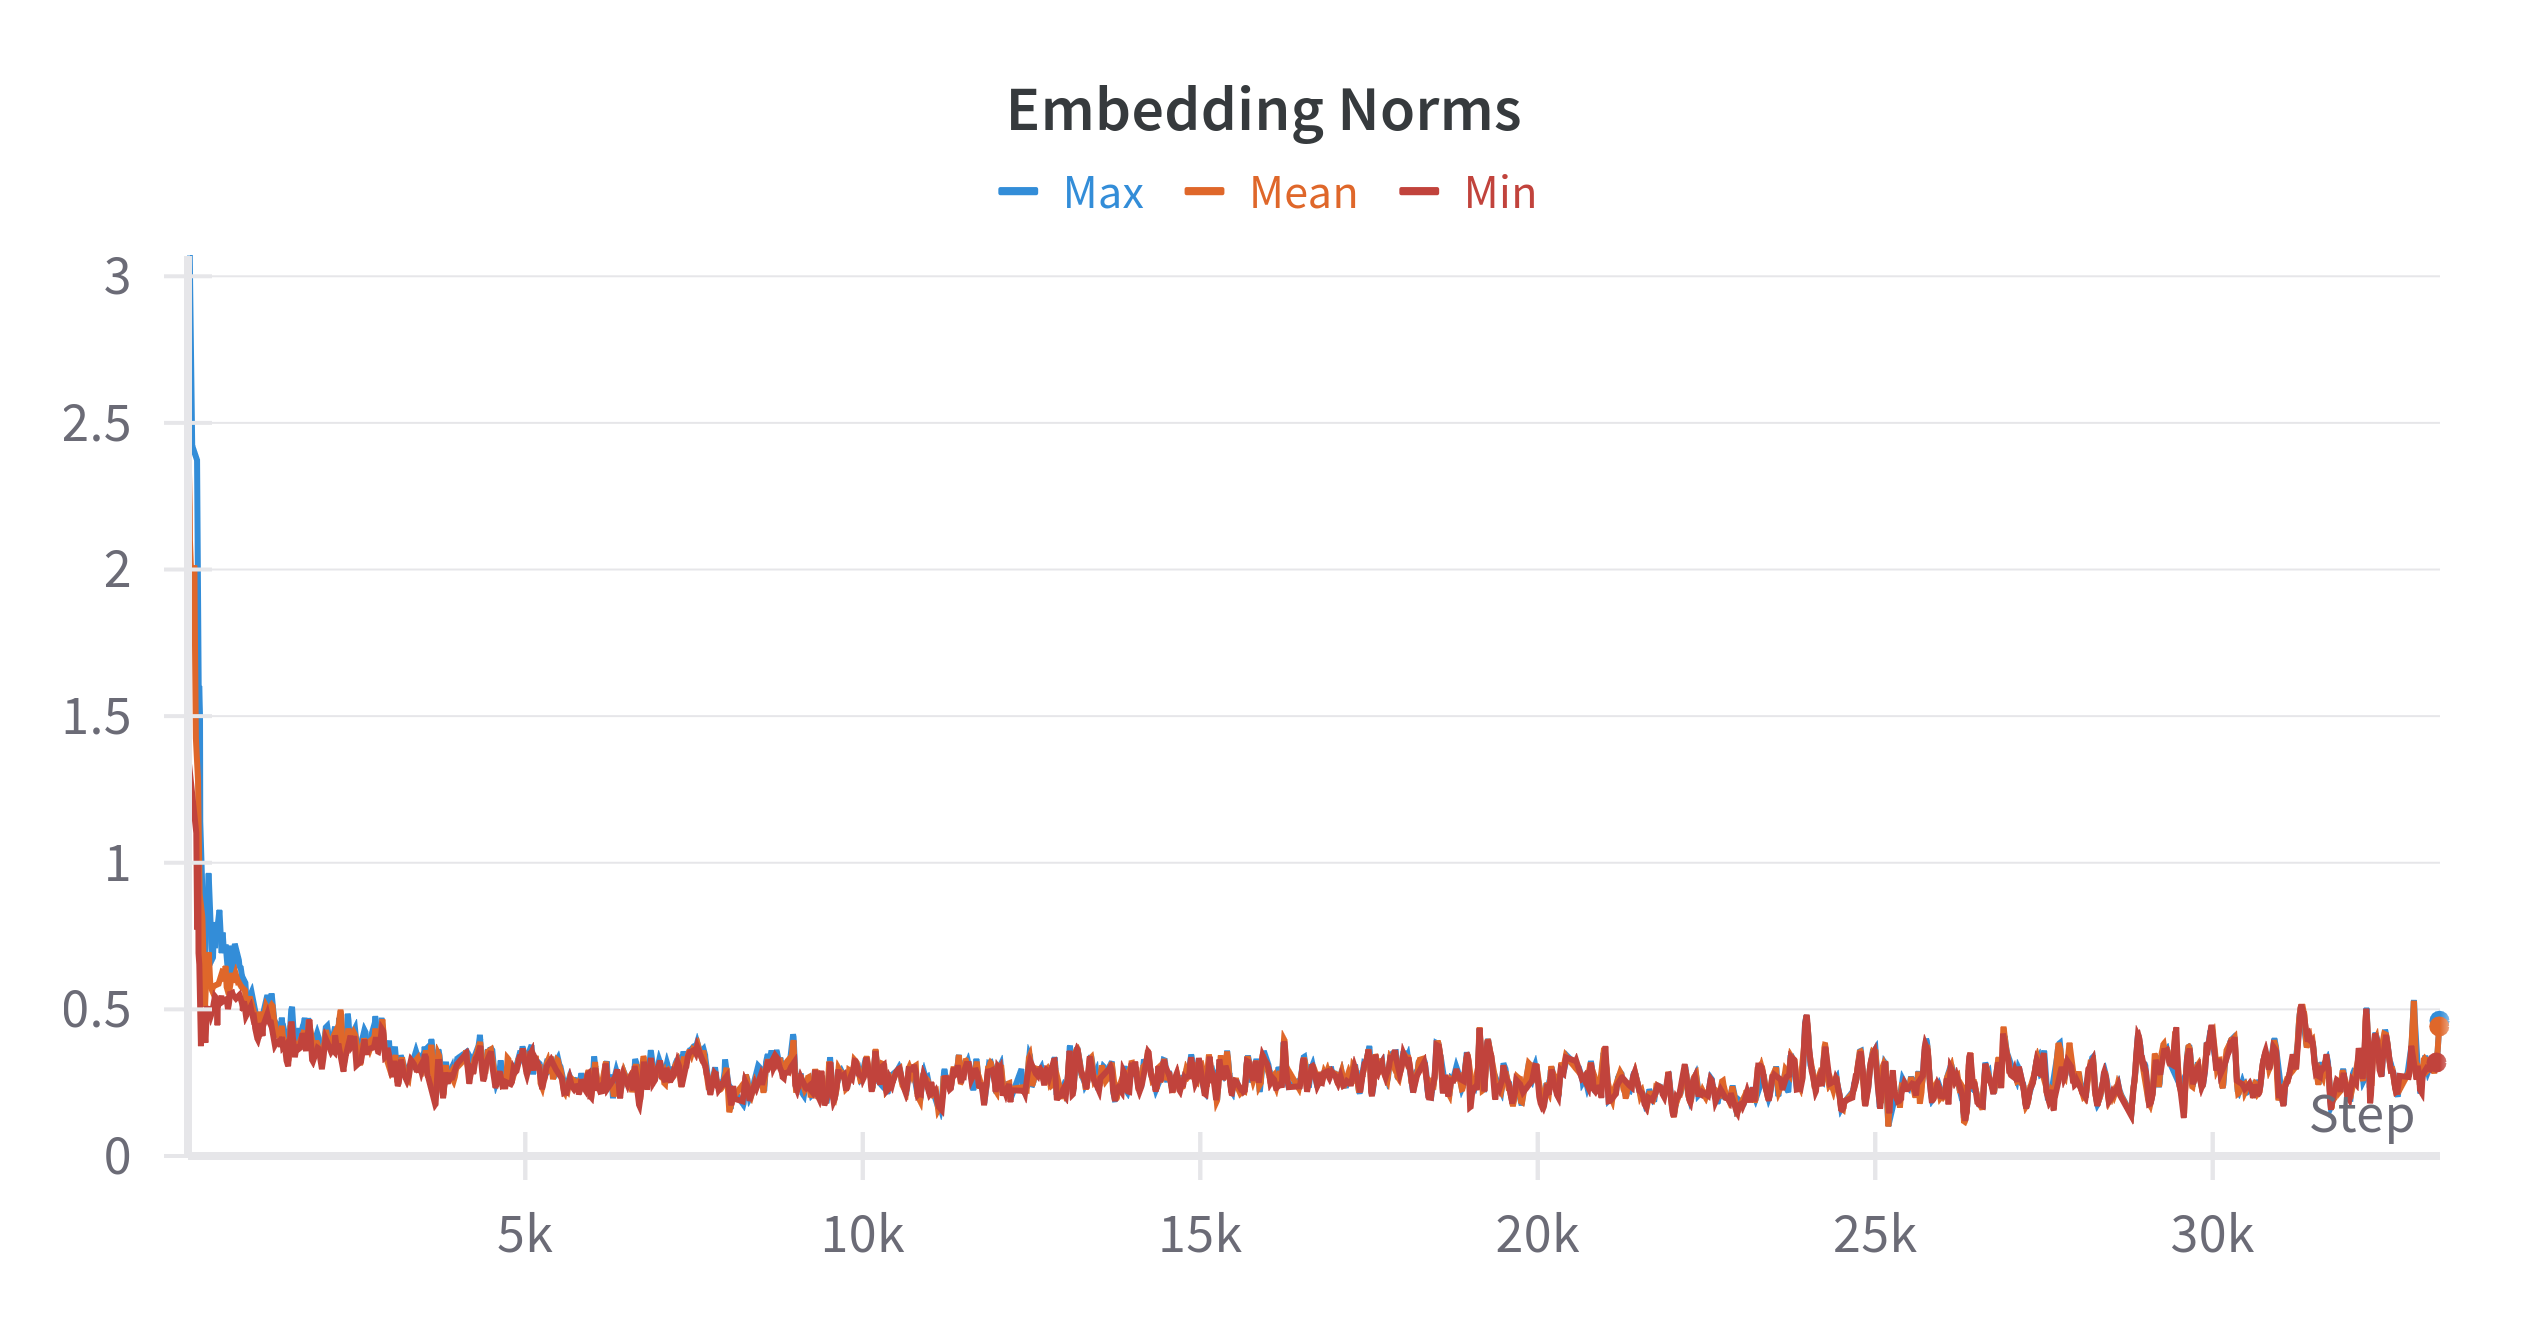
\includegraphics[width=1.0\textwidth]{informatica/wandb/entrenamiento_principal/embedding_norms}
        \caption{Norma de los \textit{embeddings}}
    \end{subfigure}

    \caption{Valores de las métricas observadas durante el proceso de entrenamiento}
    \label{img:metricas_entrenamiento}
\end{figure}

\begin{table}[!hbtp]
\centering
\begin{tabular}{|l|l|l|}
    \hline
    Métrica & Conjunto & Valor \\
    \hline

    \textit{Rank@1 Accuracy} & Entrenamiento & 0.07185 \\
    \textit{Rank@1 Accuracy} & Test & 0.01000 \\
    \textit{Rank@5 Accuracy} & Entrenamiento & 0.15244 \\
    \textit{Rank@5 Accuracy} & Test & 0.00100 \\
    \textit{Silhouette} & Entrenamiento & -0.41858 \\
    \textit{Silhouette} & Test & -0.32984 \\

    \hline

\end{tabular}
\caption{Valores de distintas métricas obtenidas sobre el conjunto \textit{CACD} de entrenamiento y sobre el conjunto \textit{FG-Net} de \textit{test}}
    \label{table:resultados_sobre_fg_net}
\end{table}

En \imgref{img:metricas_entrenamiento} podemos ver que:

\begin{itemize}
    \item Como habíamos previsto, la función de pérdida cae rápidamente mientras que el resto de métricas varían su valor. Por tanto, la red está aprendiendo cierto comportamiento (que claramente no es el deseado) aunque la función de pérdida no varíe. Esto ocurre tanto en la función de pérdida \textit{running} como en la función de pérdida computada a mano sobre los datos.
    \item Tanto el \textit{Rank@1} como \textit{Rank@5 Accuracy} aumentan satisfactoriamente, aunque sus valores son realmente bajos. Además, tenemos mejores valores en validación que en entrenamiento, lo que supone un comportamiento inusual que puede indicar que la red no está aprendiendo adecuadamente.
    \item La variante local de \textit{Rank@1} y \textit{Rank@5} obtienen resultados notablemente mejores, lo que era de esperar por la naturaleza de esta variante.
    \item Como esperábamos, la distancia intracluster desciende con el paso del tiempo. Sin embargo, la distancia intercluster desciende, en vez de ascender. Acompañado del descenso de las normas de los \textit{embeddings}, podemos pensar que estamos en la primera fase del entrenamiento que hemos comentado: agrupamos todos los datos en un cierto centro de gravedad. Pero no estamos logrando pasar a la siguiente fase, en la que se forma los clústers gracias a que los elementos atraviesen el centro de gravedad para juntarse con el resto de elementos de su clúster.
\end{itemize}

Los resultados obtenidos en \tableref{table:resultados_sobre_fg_net} muestran que:

\begin{itemize}
    \item Los resultados en el conjunto de entrenamiento son realmente malos. Los valores de \textit{Rank@1} y \textit{Rank@5 Accuracy} son pésimos, y están muy lejos de los valores que hemos mostrado que alcanzan modelos estado del arte. Aunque no logremos ser competitivos con el estado del arte, podríamos haber obtenido un modelo aplicable en la práctica, competente y ligero. Pero este no es el caso, en este estado el modelo no es aplicable en ningún escenario.
    \item En base a estos malos resultados, y como era de esperar, los valores de \textit{Rank@1} y \textit{Rank@5 Accuracy} sobre \textit{FG-Net} son pésimos.
    \item Los valores de \textit{Silhouette} son muy malos también. Un valor negativo implica que el \textit{embedding} aprendido es de una calidad pésima.
\end{itemize}

\section{Comparativas variando las técnicas empleadas} \label{isec:experimentacion_variar_tecnicas}
\todo{Desarrollar esta sección}

\section{Conclusiones extraídas de la experimentación} \label{isec:conclusiones_experimentacion}

En base a \imgref{img:metricas_entrenamiento} y \tableref{table:resultados_sobre_fg_net} queda claro que el entrenamiento de este modelo, a partir de las técnicas que hemos ido desarrollando en este trabajo, no han producido un modelo que resuelva la tarea propuesta de forma satisfactoria. En la \tableref{table:estado_del_arte_y_mi_modelo} vemos una \textbf{comparativa entre algunos modelos del estado del arte y nuestro modelo}:

\begin{table}[!hbtp]
\centering
\begin{tabular}{|l|l|}
    \hline
    Modelo                    & \textit{Rank@1 Accuracy} en \textit{FG-Net} \\
    \hline

    \textbf{\textit{MTLFace}} & \textbf{94.78}                              \\
    \textit{DAL}              & 94.5                                        \\
    \textit{AIM}              & 93.20                                       \\
    Nuestro modelo            & 0.07185                                     \\
    \hline

\end{tabular}
\caption{Resultados \textit{Rank@1 Accuracy} de distintos modelos del estado del arte y el modelo que hemos entrenado en este trabajo}
\label{table:estado_del_arte_y_mi_modelo}
\end{table}

Claramente, \textbf{nuestro modelo está muy lejos de ser competitivo con los modelos del estado del arte}. Es más, está \textbf{lejos de ser aplicable en ningún escenario práctico}. Podríamos haber obtenido un modelo que, aunque no fuera competitivo con el estado del arte, tuviese un rendimiento decente. En cuyo caso tendríamos un modelo aplicable mucho más ligero que los modelos del estado del arte. Pero estamos muy lejos de encontrarnos en esa situación.

El rendimiento ha sido tan malo que hemos pensado que existía un error en nuestra extensa base de código. Esto ha motivado la implementación de una amplia gama de \textit{tests} para descartar esta opción, como hemos desarrollado en \sectionref{isec:test_suite}. Gracias a esta amplia \textit{suite} de \textit{tests} descartamos, con cierto grado de confianza, que los malos resultados se deban a un error de implementación.

Los resultados son tan malos que \textbf{no consideramos que merezca la pena realizar modificaciones a las técnicas empleadas}, basadas en \textit{triplet loss}, para buscar mejoras futuras de rendimiento. En base a estos resultados, el enfoque más adecuado sería explorar técnicas radicalmente diferentes, como las propuestas por los distintos modelos del estado del arte que hemos estudiado en \sectionref{isec:mejores_modelos_estado_arte}.
